\documentclass[a4paper,12pt]{article}

\usepackage{graphicx}
\usepackage{amsmath}
\usepackage{hyperref}
\usepackage{caption}
\usepackage{subcaption}

\title{\textbf{Lab Report: Experiment 1}}
\author{EE24BTECH11003 : Akshara Sarma Chennubhatla\\EE24BTECH11005 : Arjun Pavanje}

\begin{document}
\maketitle
\begin{center}
	\textbf{Experiment:}\\Plotting Lissajous Figures\\and Capturing One-Time Events\\on an Oscilloscope
\end{center}
\vspace{30pt}
\begin{figure}[h!]
	\centering
	
\includegraphics[width = 100pt]{.logo/logo.png}\\
\end{figure}
\vspace{50pt}
\begin{center}
Bachelor of Technology\\
\vspace{10pt}
Department of Electrical Engineering\\
\end{center}
\newpage
\section*{Objective}
1. To observe and analyze at least 6 Lissajous figures using an oscilloscope and justify their patterns with Python codes.\\
2. To demonstrate the method to capture a one-time event.\\

\section*{Equipment Used}
\begin{itemize}
\item \text{Oscilloscope}
    \item \text{Function generator}
    \item \text{Oscilloscope probes and cables}
\end{itemize}
\section*{Theory}
\subsection*{Lissajous Figures}
Say we are given two waveforms defined by,
\begin{align*}
  x(t) = f_x(t, A_x, \omega _x, \phi _x)\\
  y(t) = f_y(t, A_y, \omega _y, \phi_y)
\end{align*}
Where $A, \omega, \phi$ represent Amplitude, Angular Frequency, Initial Phase respectively. A Lissajous figure is the graph obtained by plotting $x(t)$ against $y(t)$. \newline
For sinusoidal waveforms, 
\begin{align*}
  x(t) = A \sin (\omega t + \phi)
\end{align*}
and for ramp waveforms, one way of representing them is, 
\begin{align*}
  x(t) = (\frac{2A}{\pi} \cos^{-1}cos(\omega t + \phi)) - A
  \end{align*}
  Ramp waveforms may also be defined as a piece-wise function, but this is what we have used in our python code to verify. To verify results, we can obtain the points in $x(t), y(t)$ and plot them against each other.
\section*{Procedure}

\subsection*{Plotting of Lissajous Figures}
\begin{enumerate}
	\item Connect the two input channels of the function generator to the two reciever channels of the oscilloscope.
	\item For each channel, connect the positive end of the cable from the function generator to the positive end of the probe and the other (ground) end to the ground of the probe
	\item Set the function generator to produce sinusoidal (or ramp) waveforms on both channels of varying phase, amplitude, frequency.
	\item Use the phase alignment feature of the function generator to ensure that both waveforms start at the same time.
	\item Record and analyze the patterns observed on the oscilloscope.
	\item Repeat the process for at least six different sets of waveforms in which the amplitude, starting-phase, frequency, wave-type (ramp or sinusoidal) parameters are varied
\end{enumerate}

\subsection*{Capturing One-Time Events}
\begin{enumerate}
    	\item In the function generator, select a square wave (alternatively, a ramp or sine function may also be used) as the waveform.
    	\item Press the \textit{MOD} button and choose the \textit{BURST} option. Set the trigger to manual.
	\item Select the type of cycle as \textit{N-CYCLES}.
    	\item This configuration enables the generation of a square wave with a predefined number of cycles when the trigger button is pressed on the function generator.
    	\item Connect the function generator to the oscilloscope.
	\item On the oscilloscope, press the \textit{SINGLE} button. This ensures that the next event captured by the oscilloscope is displayed and then the display pauses automatically.
    	\item Trigger the burst mode manually on the function generator to generate the single pulse or event.
    	\item Observe and record the captured waveform on the oscilloscope.
\end{enumerate}
\section*{Results and Verification}
We have written the code in python to plot the same figures to verify if the figures obtained on the oscilloscope are correct or not.\\

\subsection*{Lissajous Figures}
\begin{enumerate}
	\item $x(t) = 13\sin(2000\pi\omega t + \frac{\pi}{3})$, $y(t) = 4\sin(10000\pi\omega t + \frac{5\pi}{9})$\\
\begin{figure}[h!]
	\begin{subfigure}[b]{10pt}
		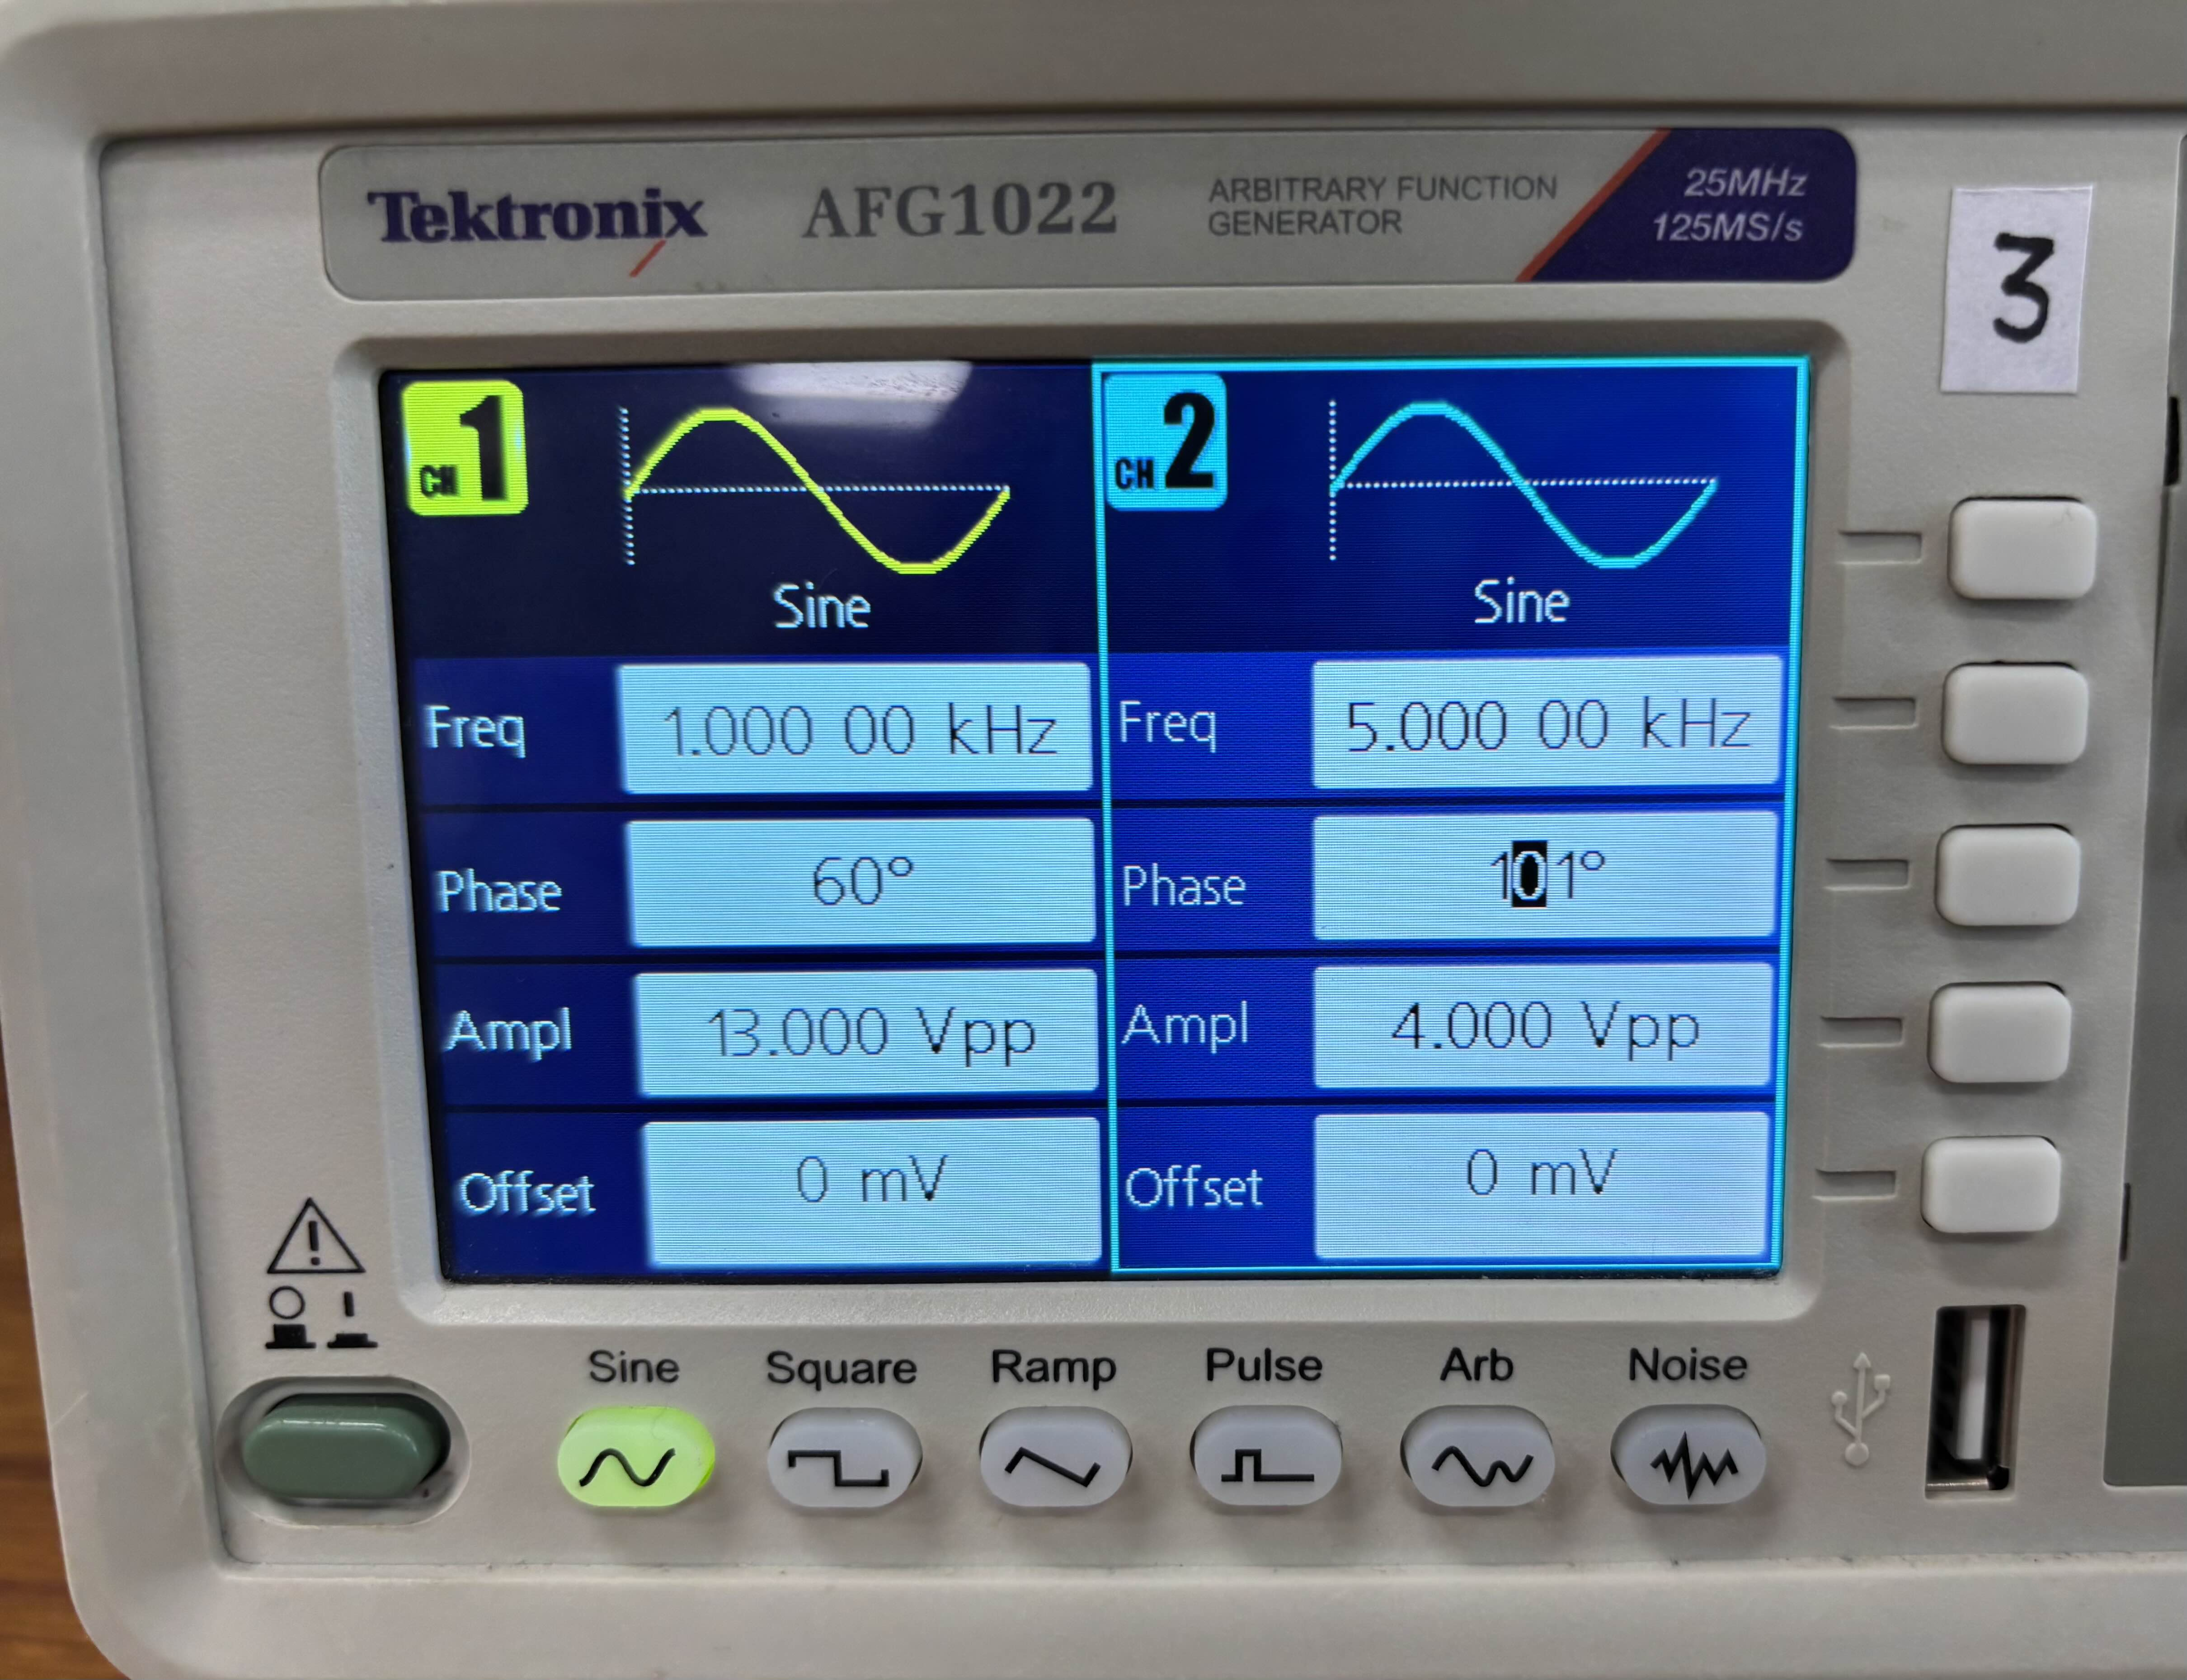
\includegraphics[width = 150pt]{figs/fig1.jpeg}
	\end{subfigure}
	\hspace{135pt}
	\begin{subfigure}[b]{10pt}
		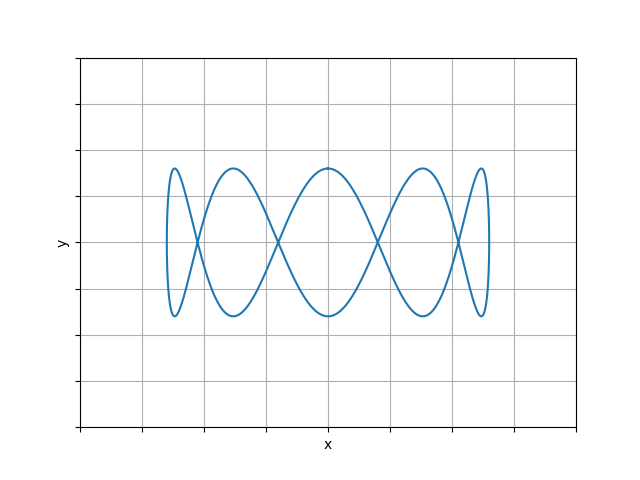
\includegraphics[width = 150pt]{figs/fig1.png}
	\end{subfigure}
	\hspace{135pt}
	\begin{subfigure}[b]{10pt}
		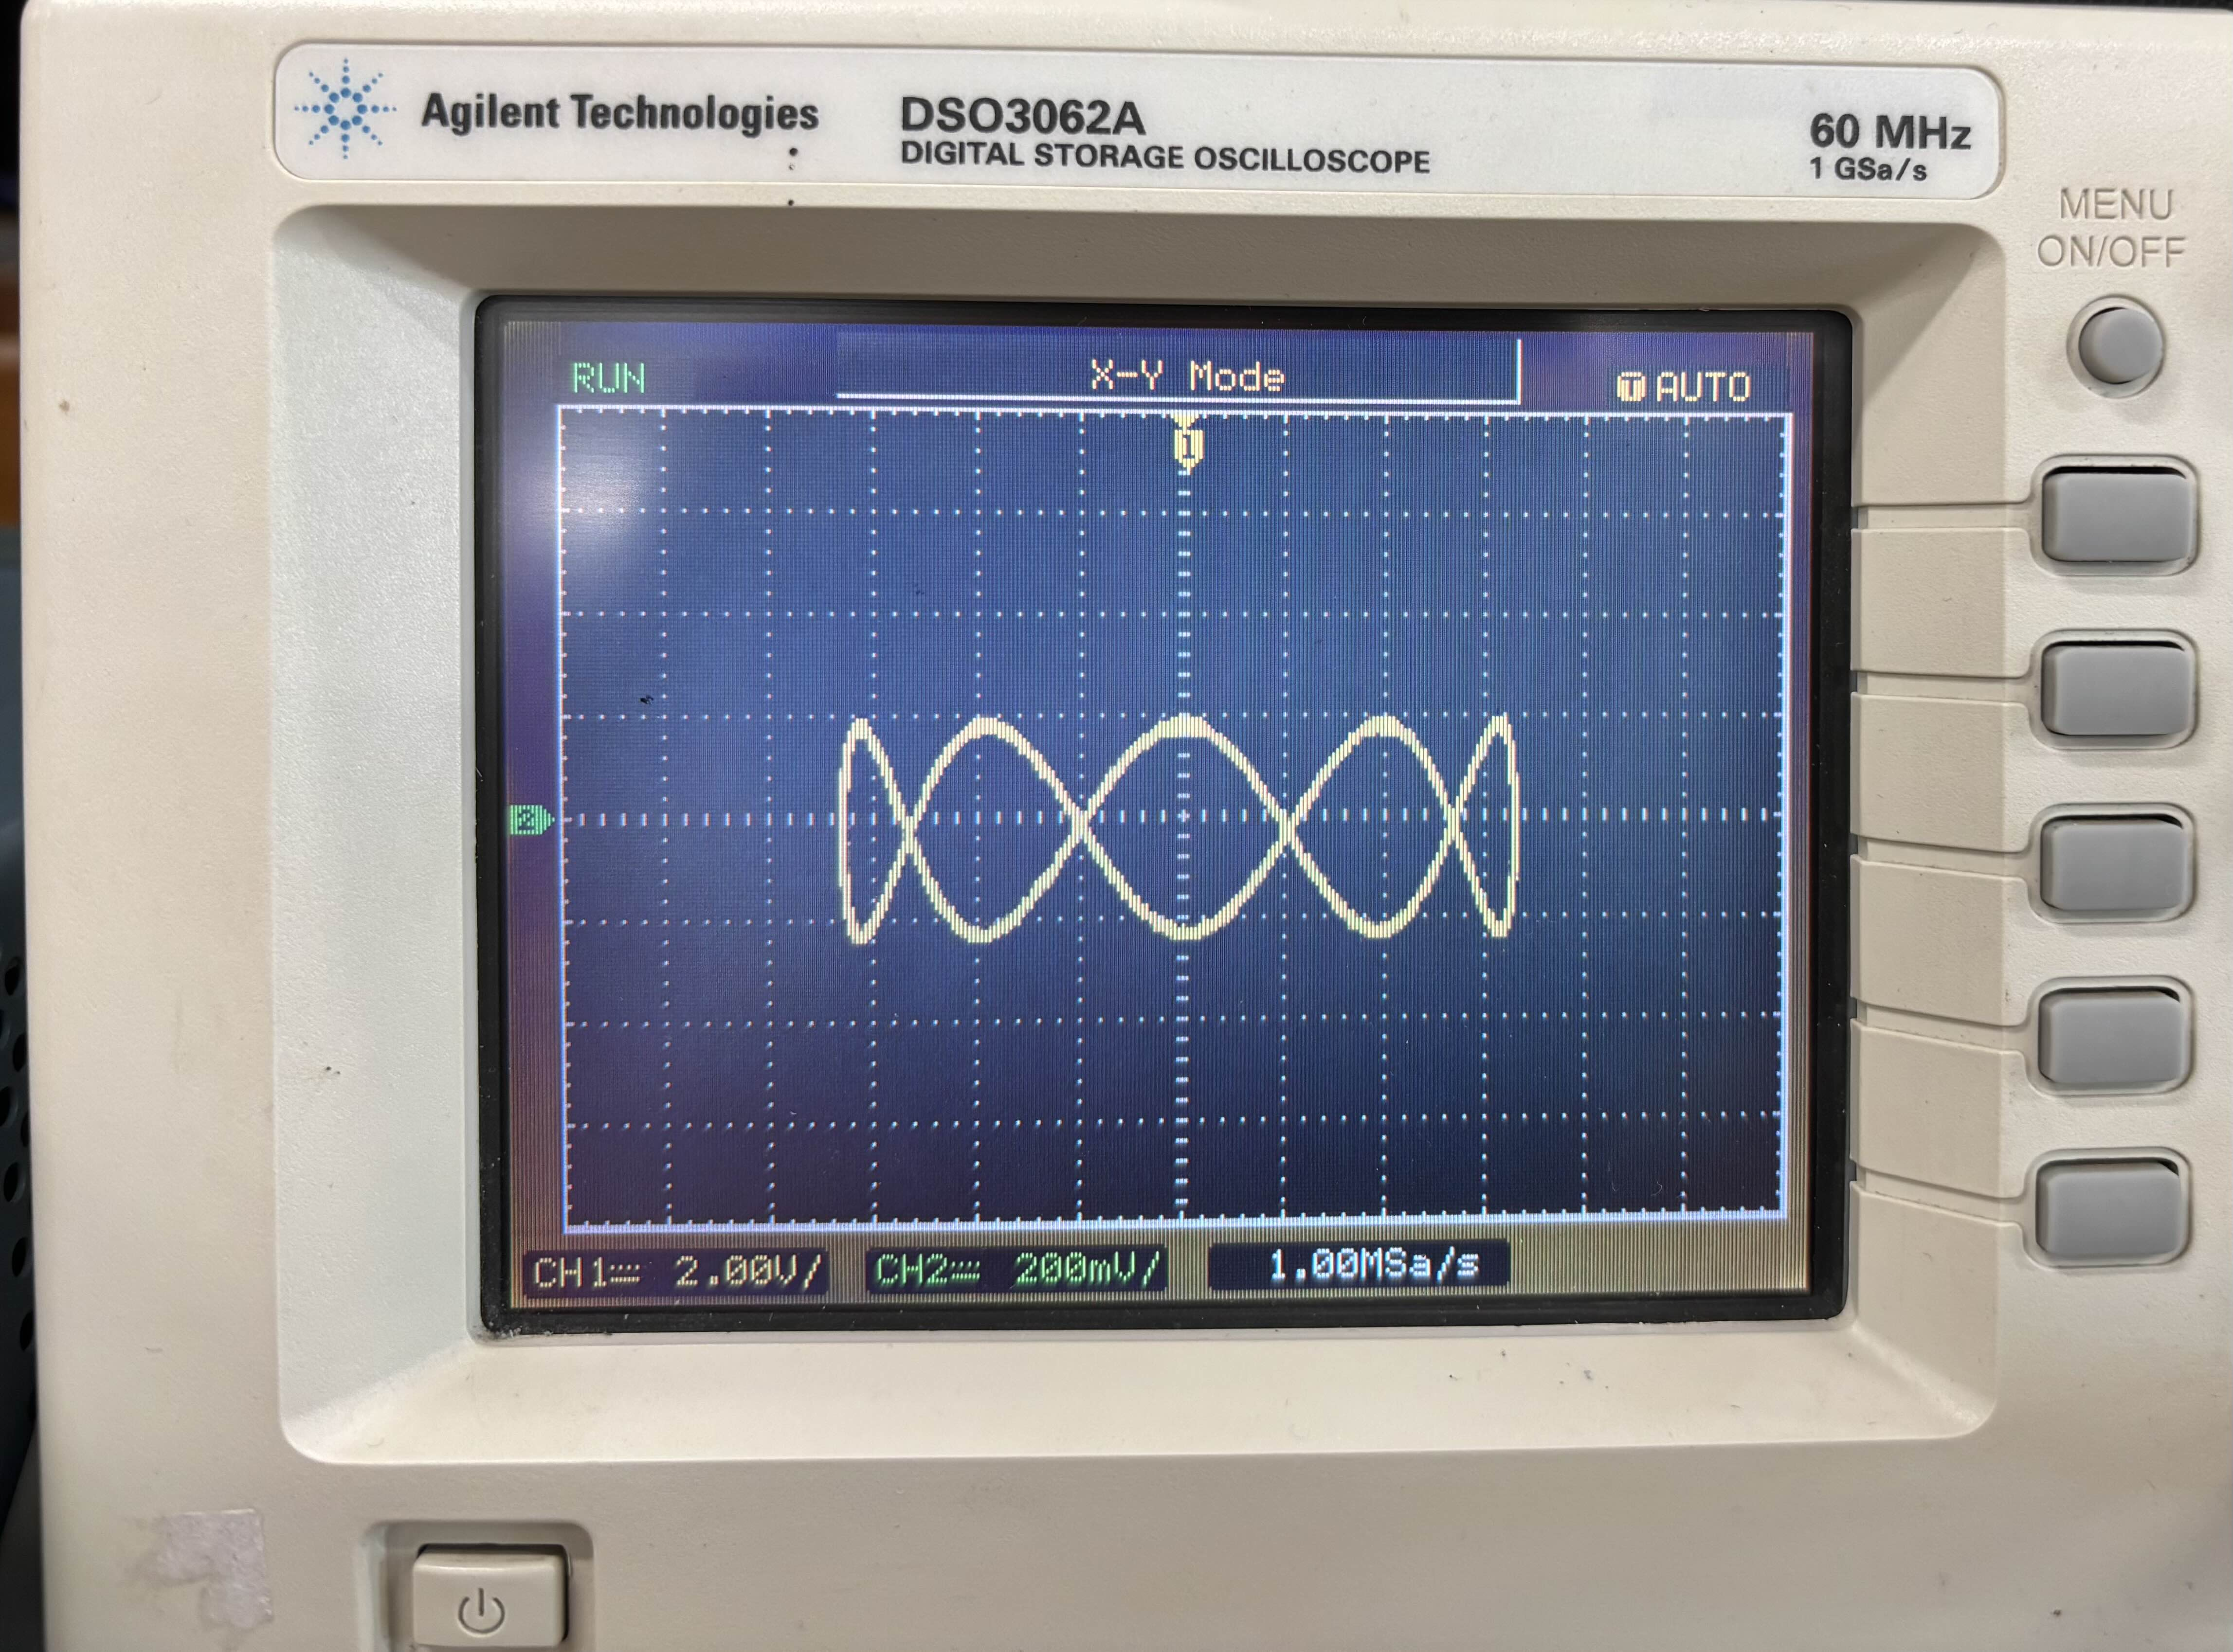
\includegraphics[width = 150pt]{figs/fig1_1.jpeg}
	\end{subfigure}
	\caption{Lissajous Figure 1}
\end{figure}
\pagebreak
	\item $x(t) = 7\sin(2000\pi\omega t + \frac{\pi}{2})$, $y(t) = 7\sin(1000\pi\omega t)$\\
\begin{figure}[h!]
	\begin{subfigure}[b]{10pt}
		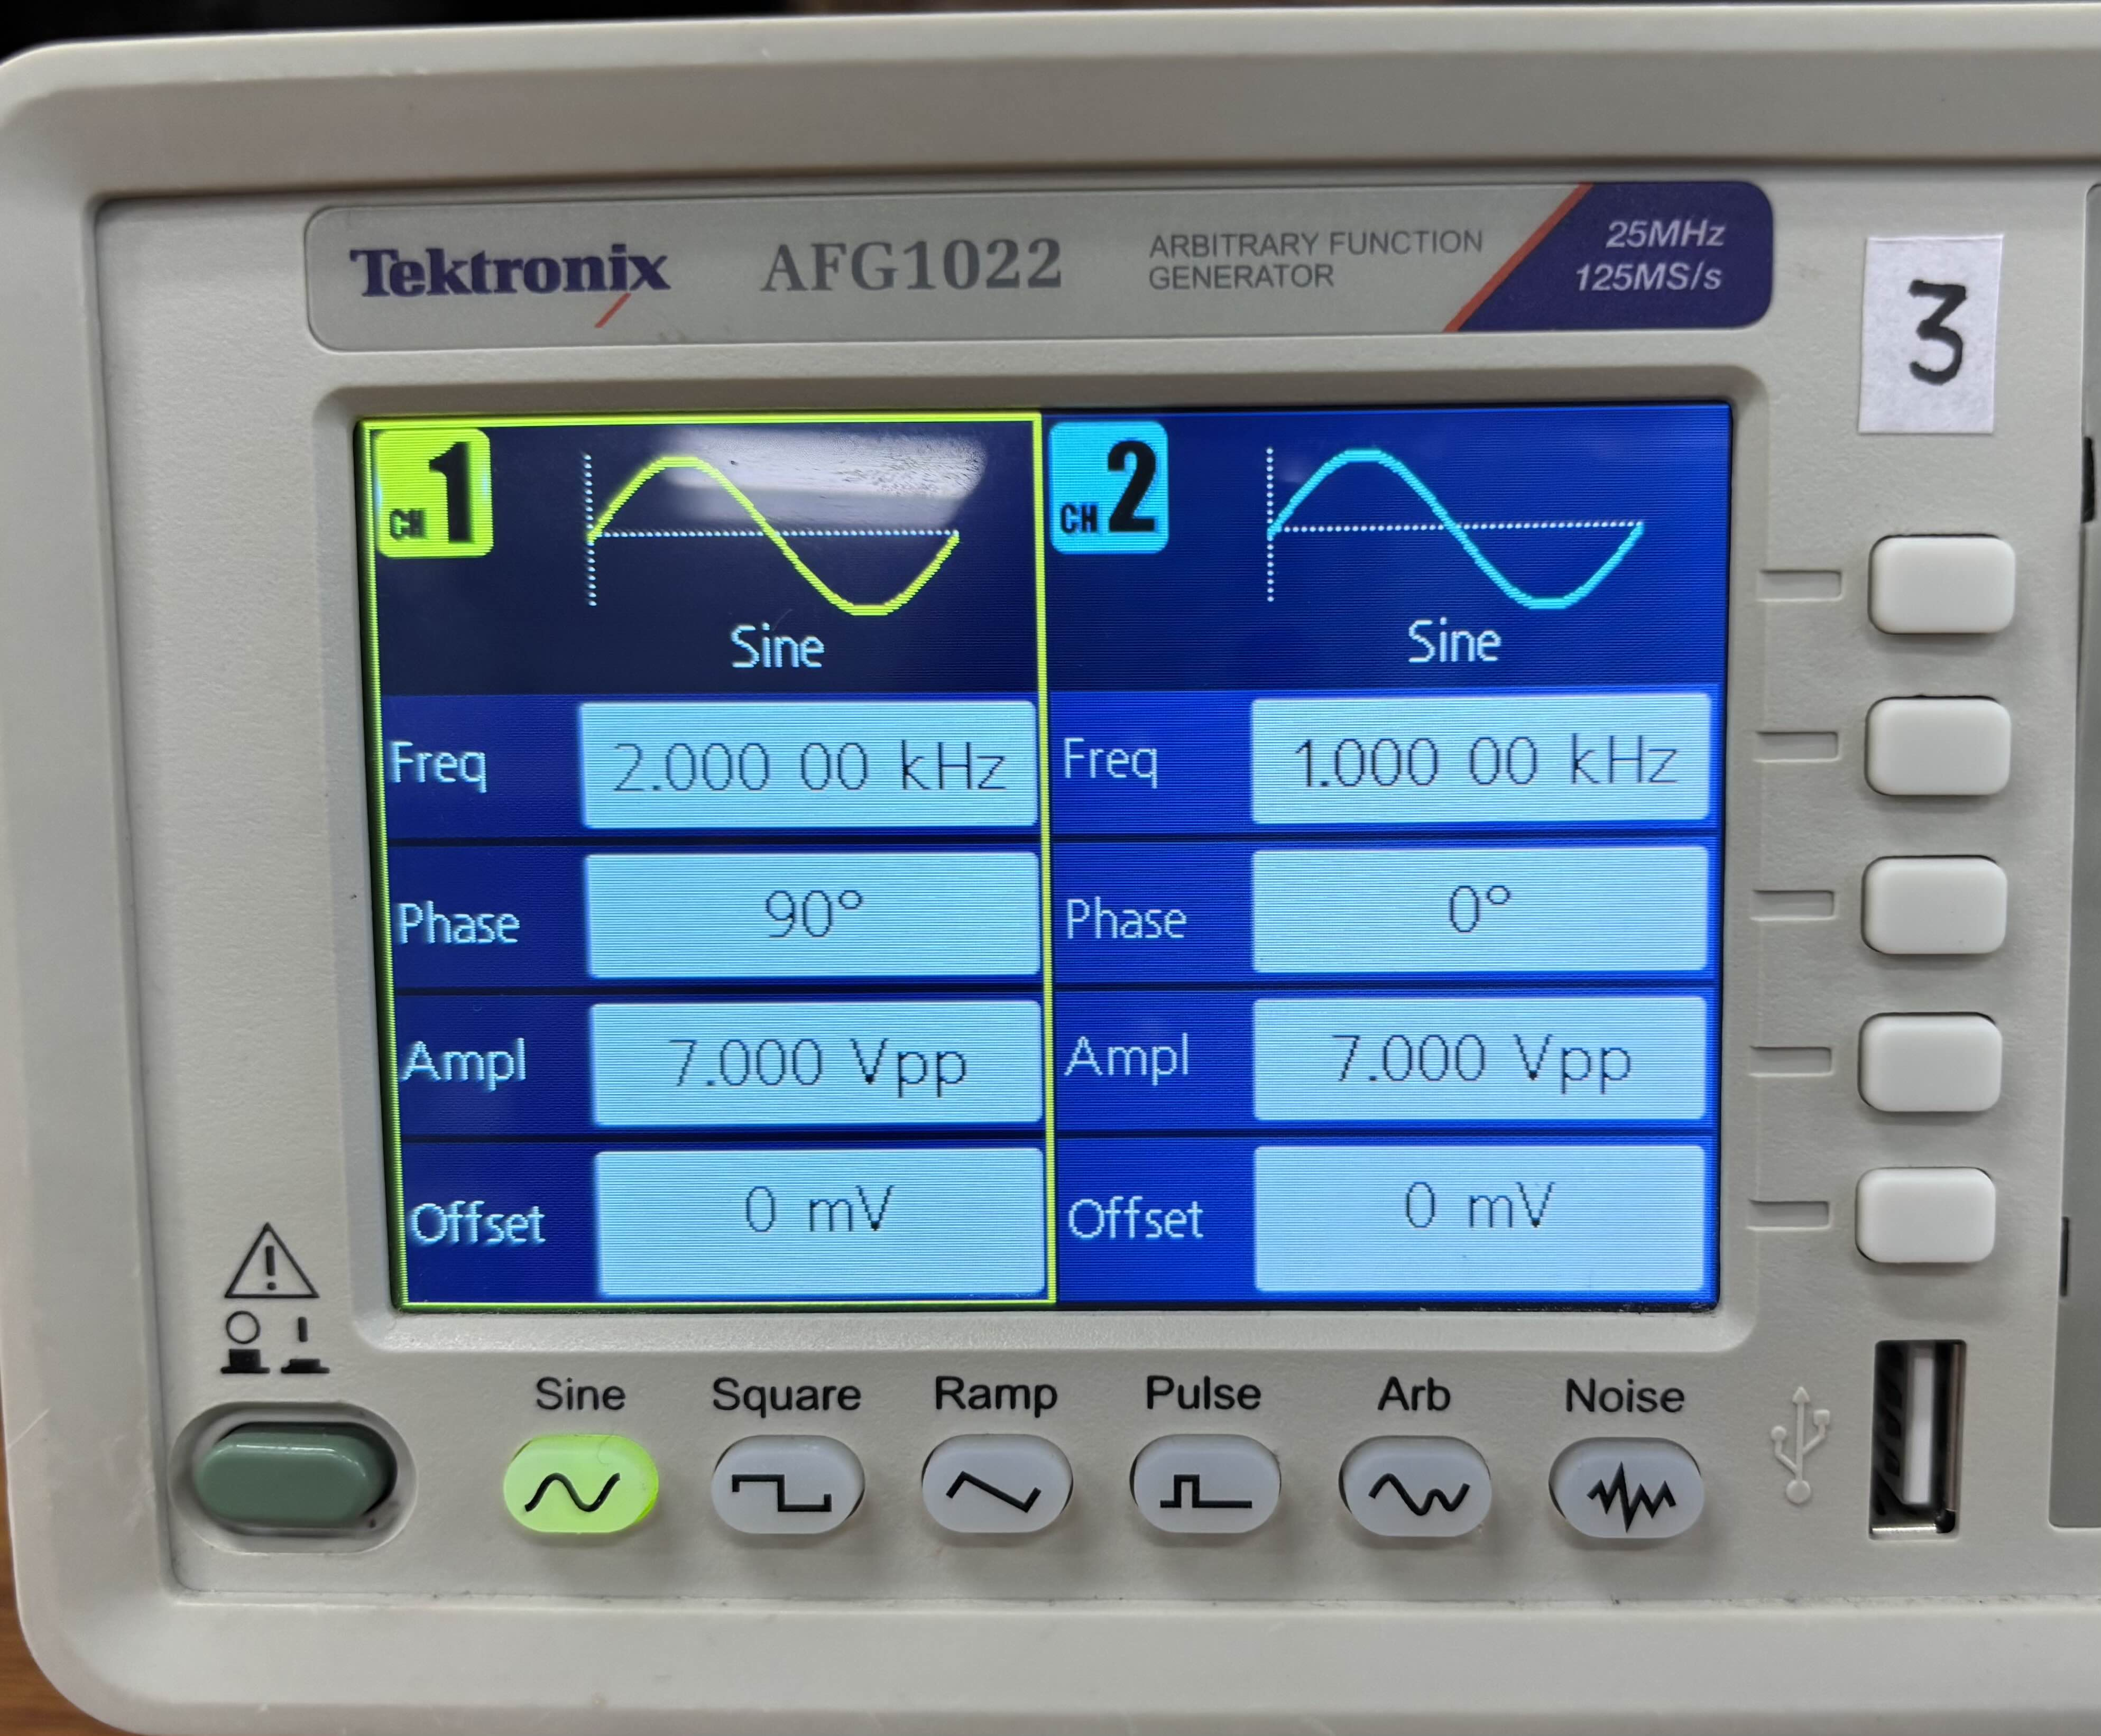
\includegraphics[width = 150pt]{figs/fig2.jpeg}
	\end{subfigure}
	\hspace{135pt}
	\begin{subfigure}[b]{10pt}
		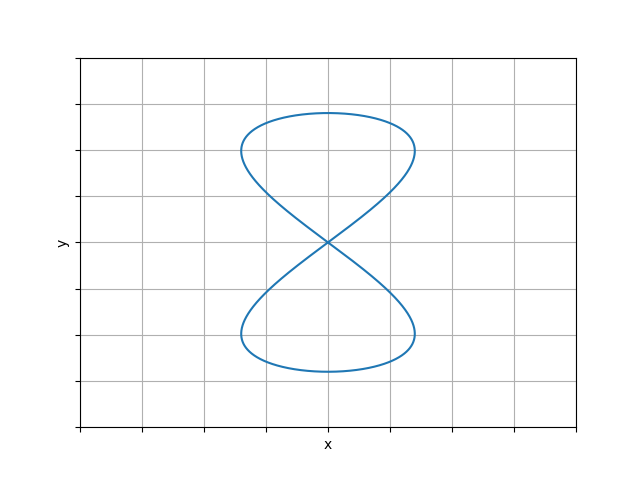
\includegraphics[width = 150pt]{figs/fig2.png}
	\end{subfigure}
	\hspace{135pt}
	\begin{subfigure}[b]{10pt}
		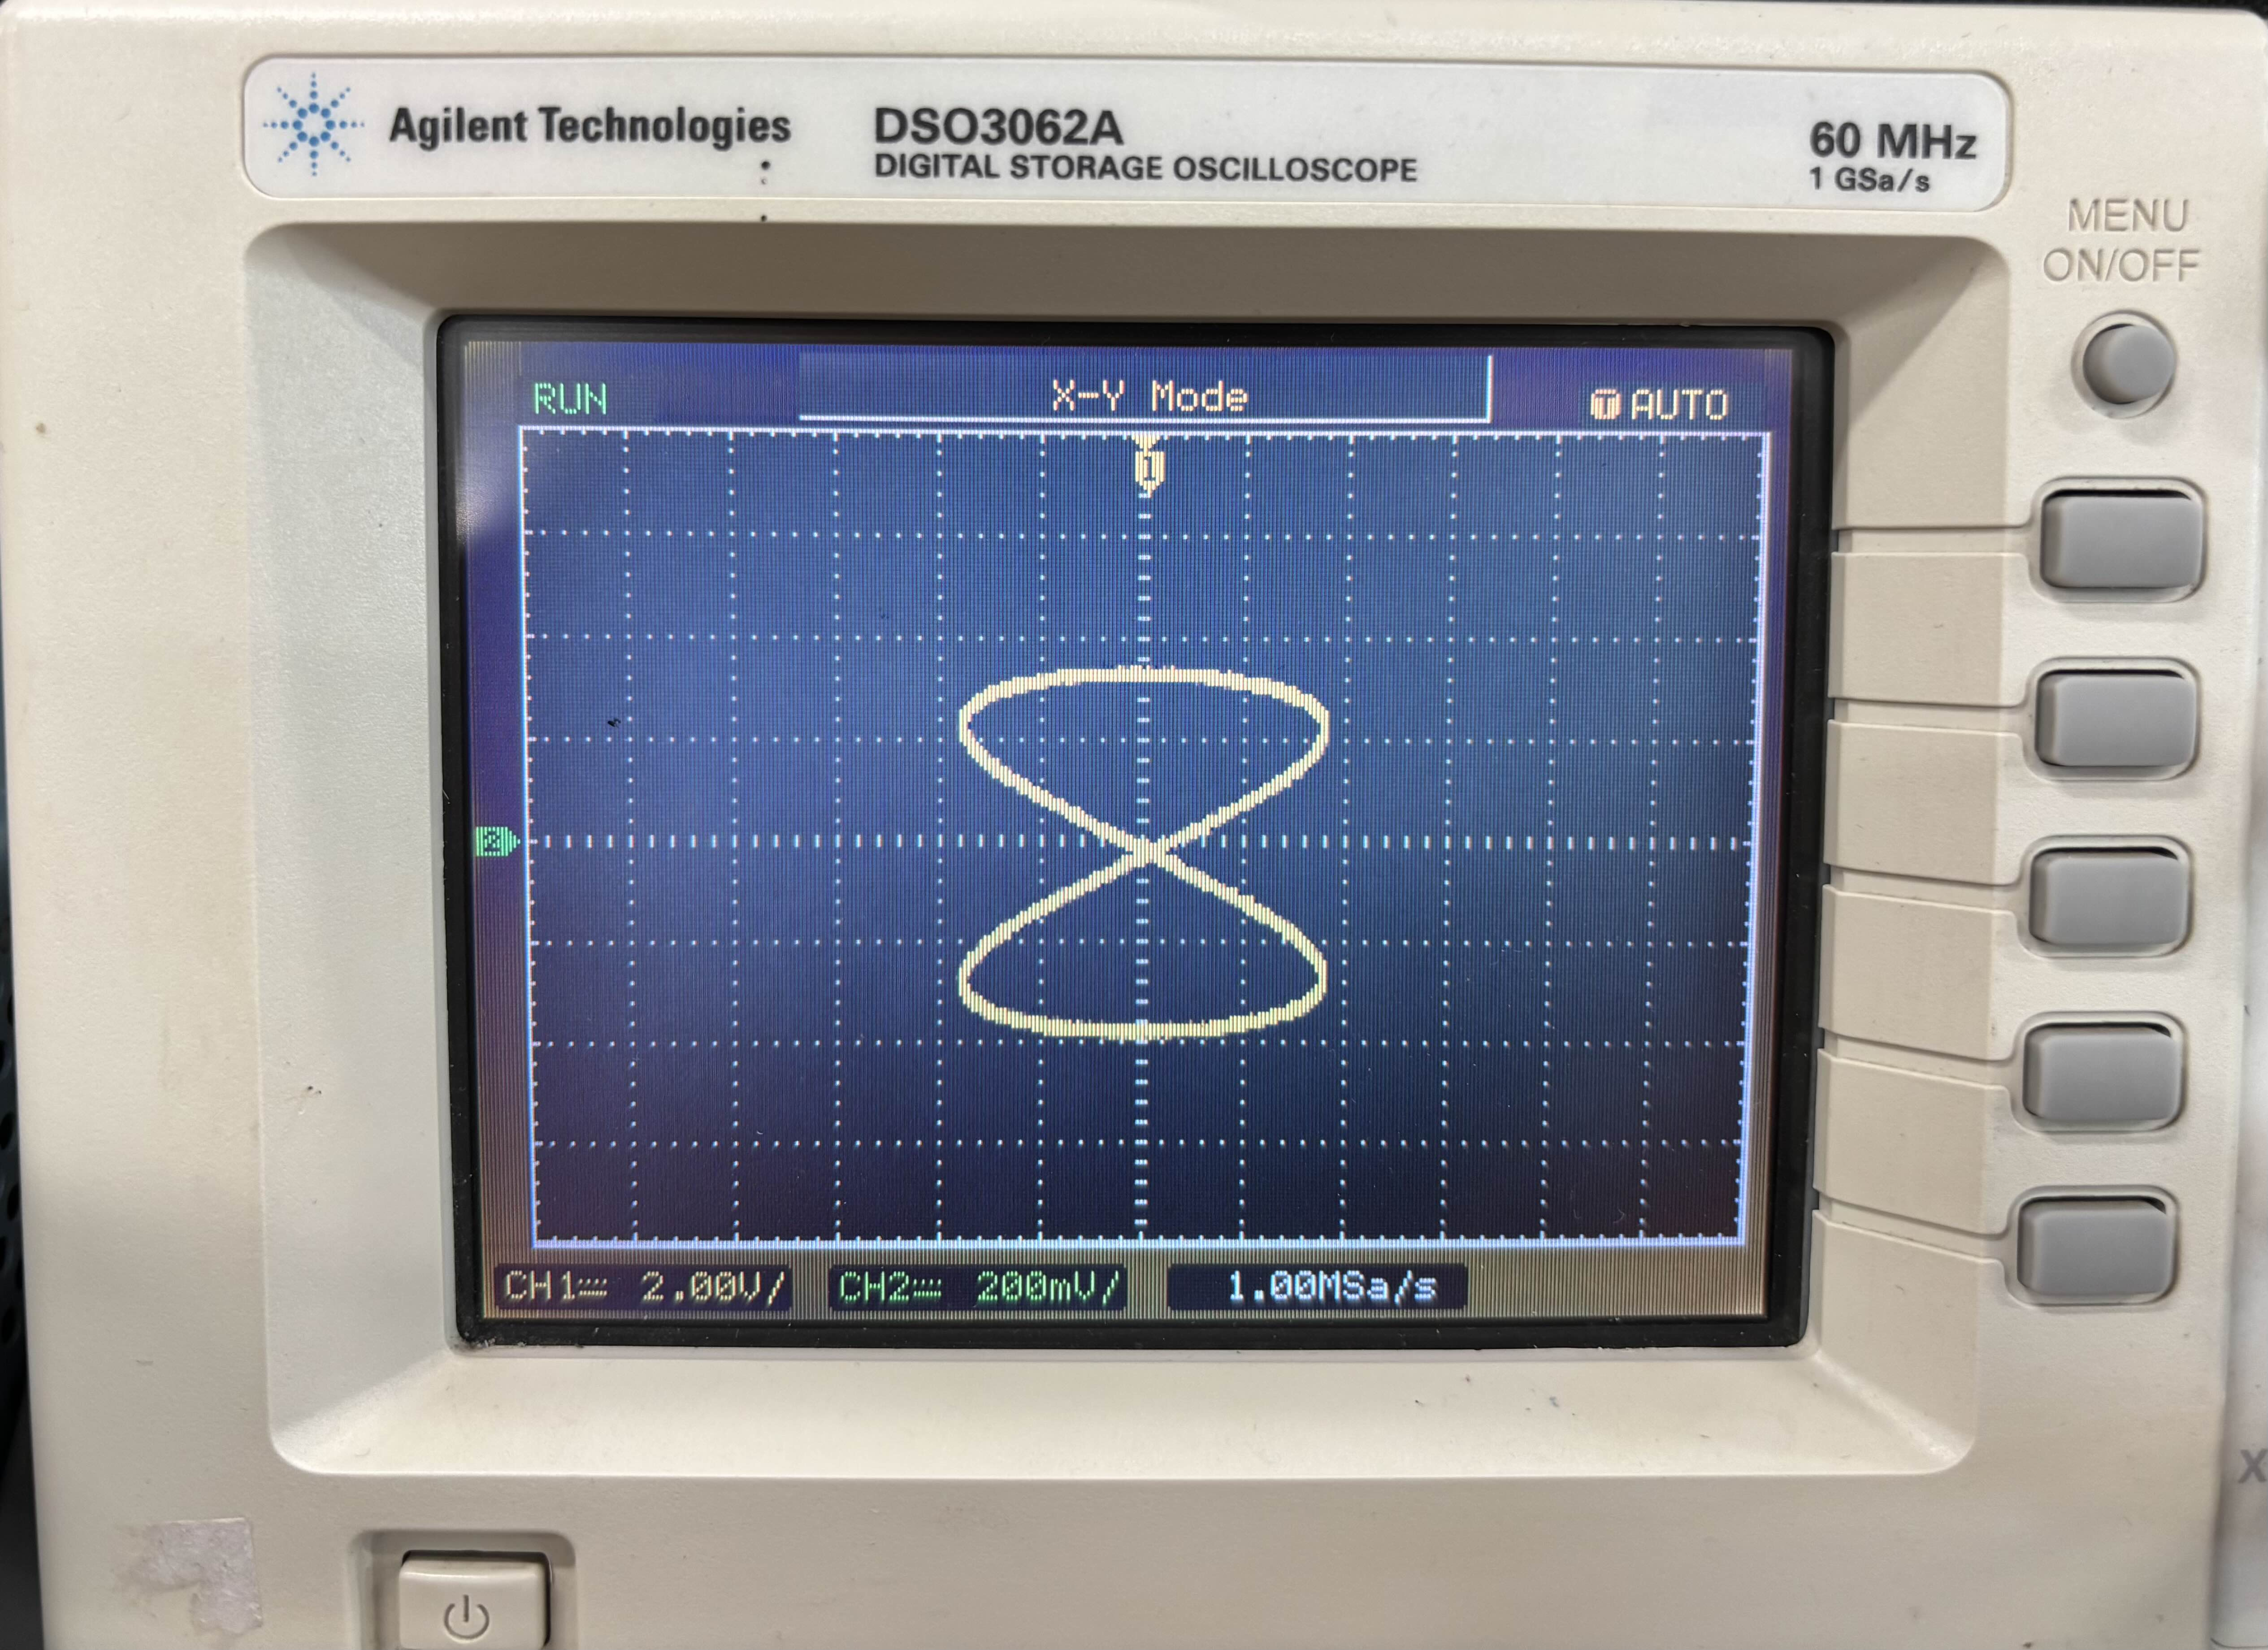
\includegraphics[width = 150pt]{figs/fig2_1.jpeg}
	\end{subfigure}
	\caption{Lissajous Figure 2}
\end{figure}
	\item $x(t) = 7\sin(1000\pi\omega t + \frac{\pi}{3})$, $y(t) = 7\sin(1000\pi\omega t)$\\
\begin{figure}[h!]
	\begin{subfigure}[b]{10pt}
		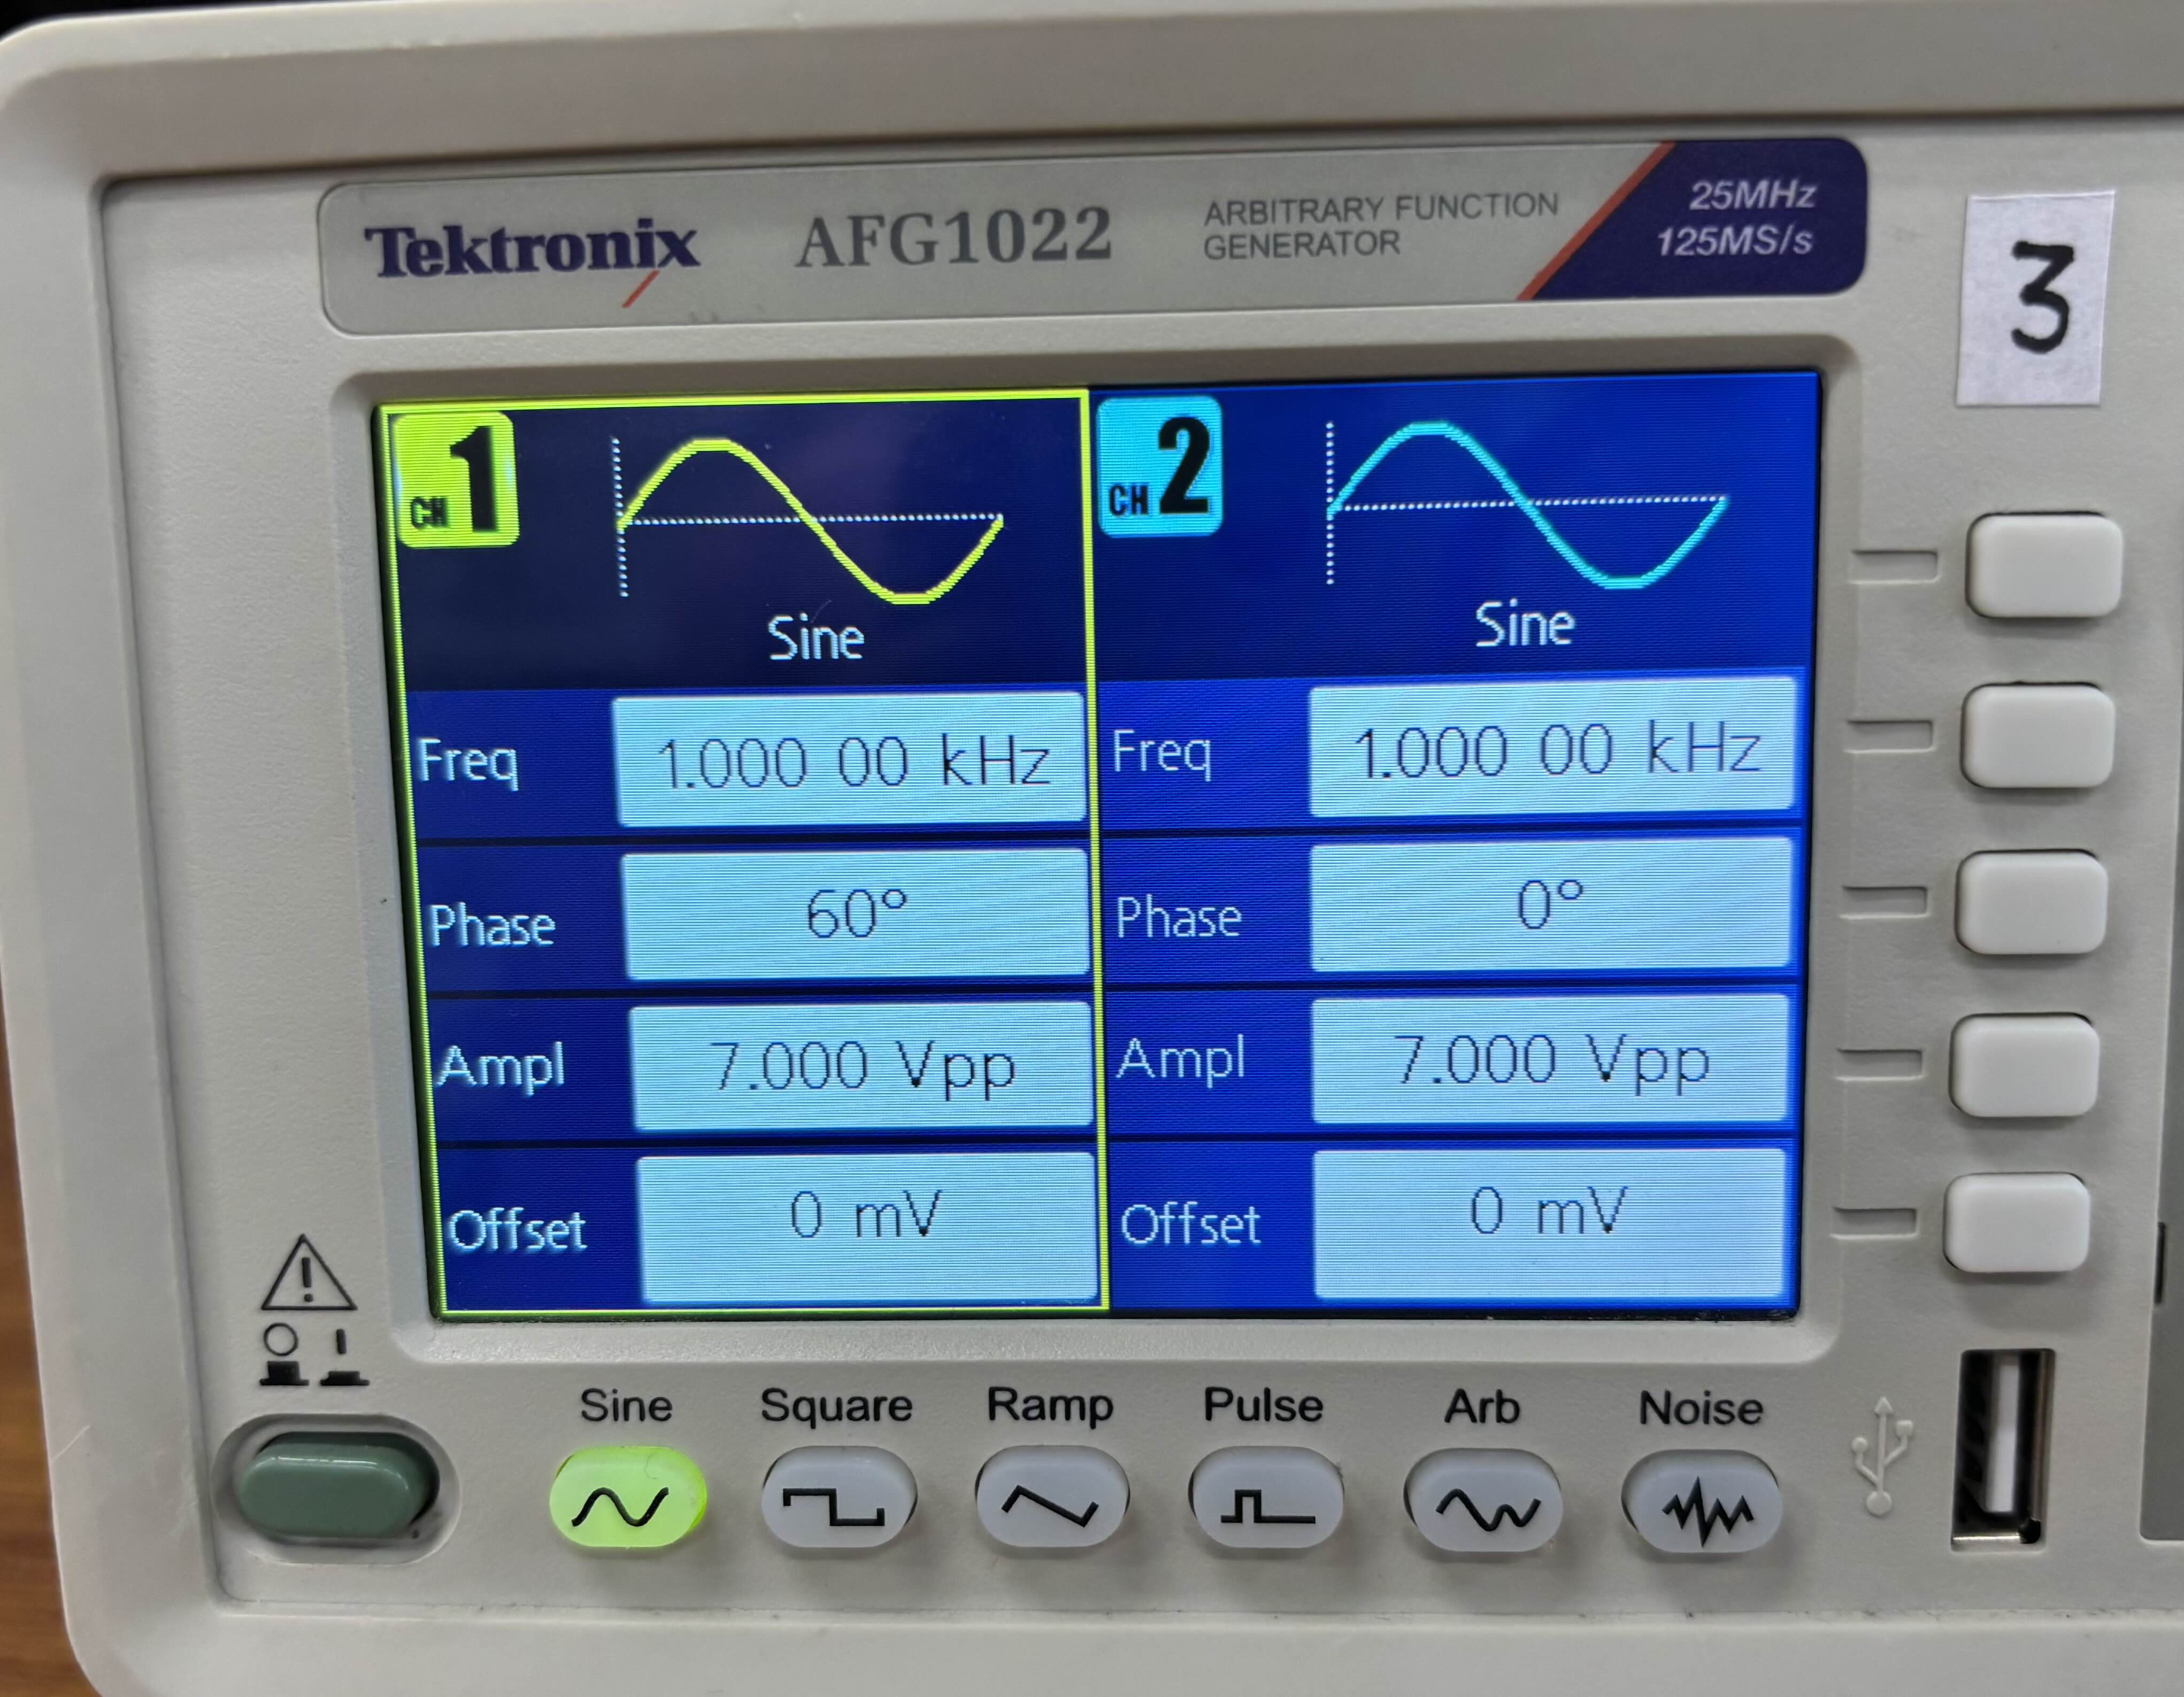
\includegraphics[width = 150pt]{figs/fig3.jpeg}
	\end{subfigure}
	\hspace{135pt}
	\begin{subfigure}[b]{10pt}
		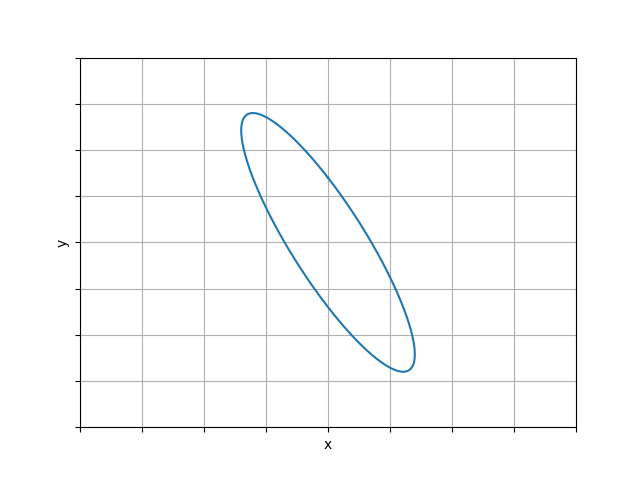
\includegraphics[width = 150pt]{figs/fig3.png}
	\end{subfigure}
	\hspace{135pt}
	\begin{subfigure}[b]{10pt}
		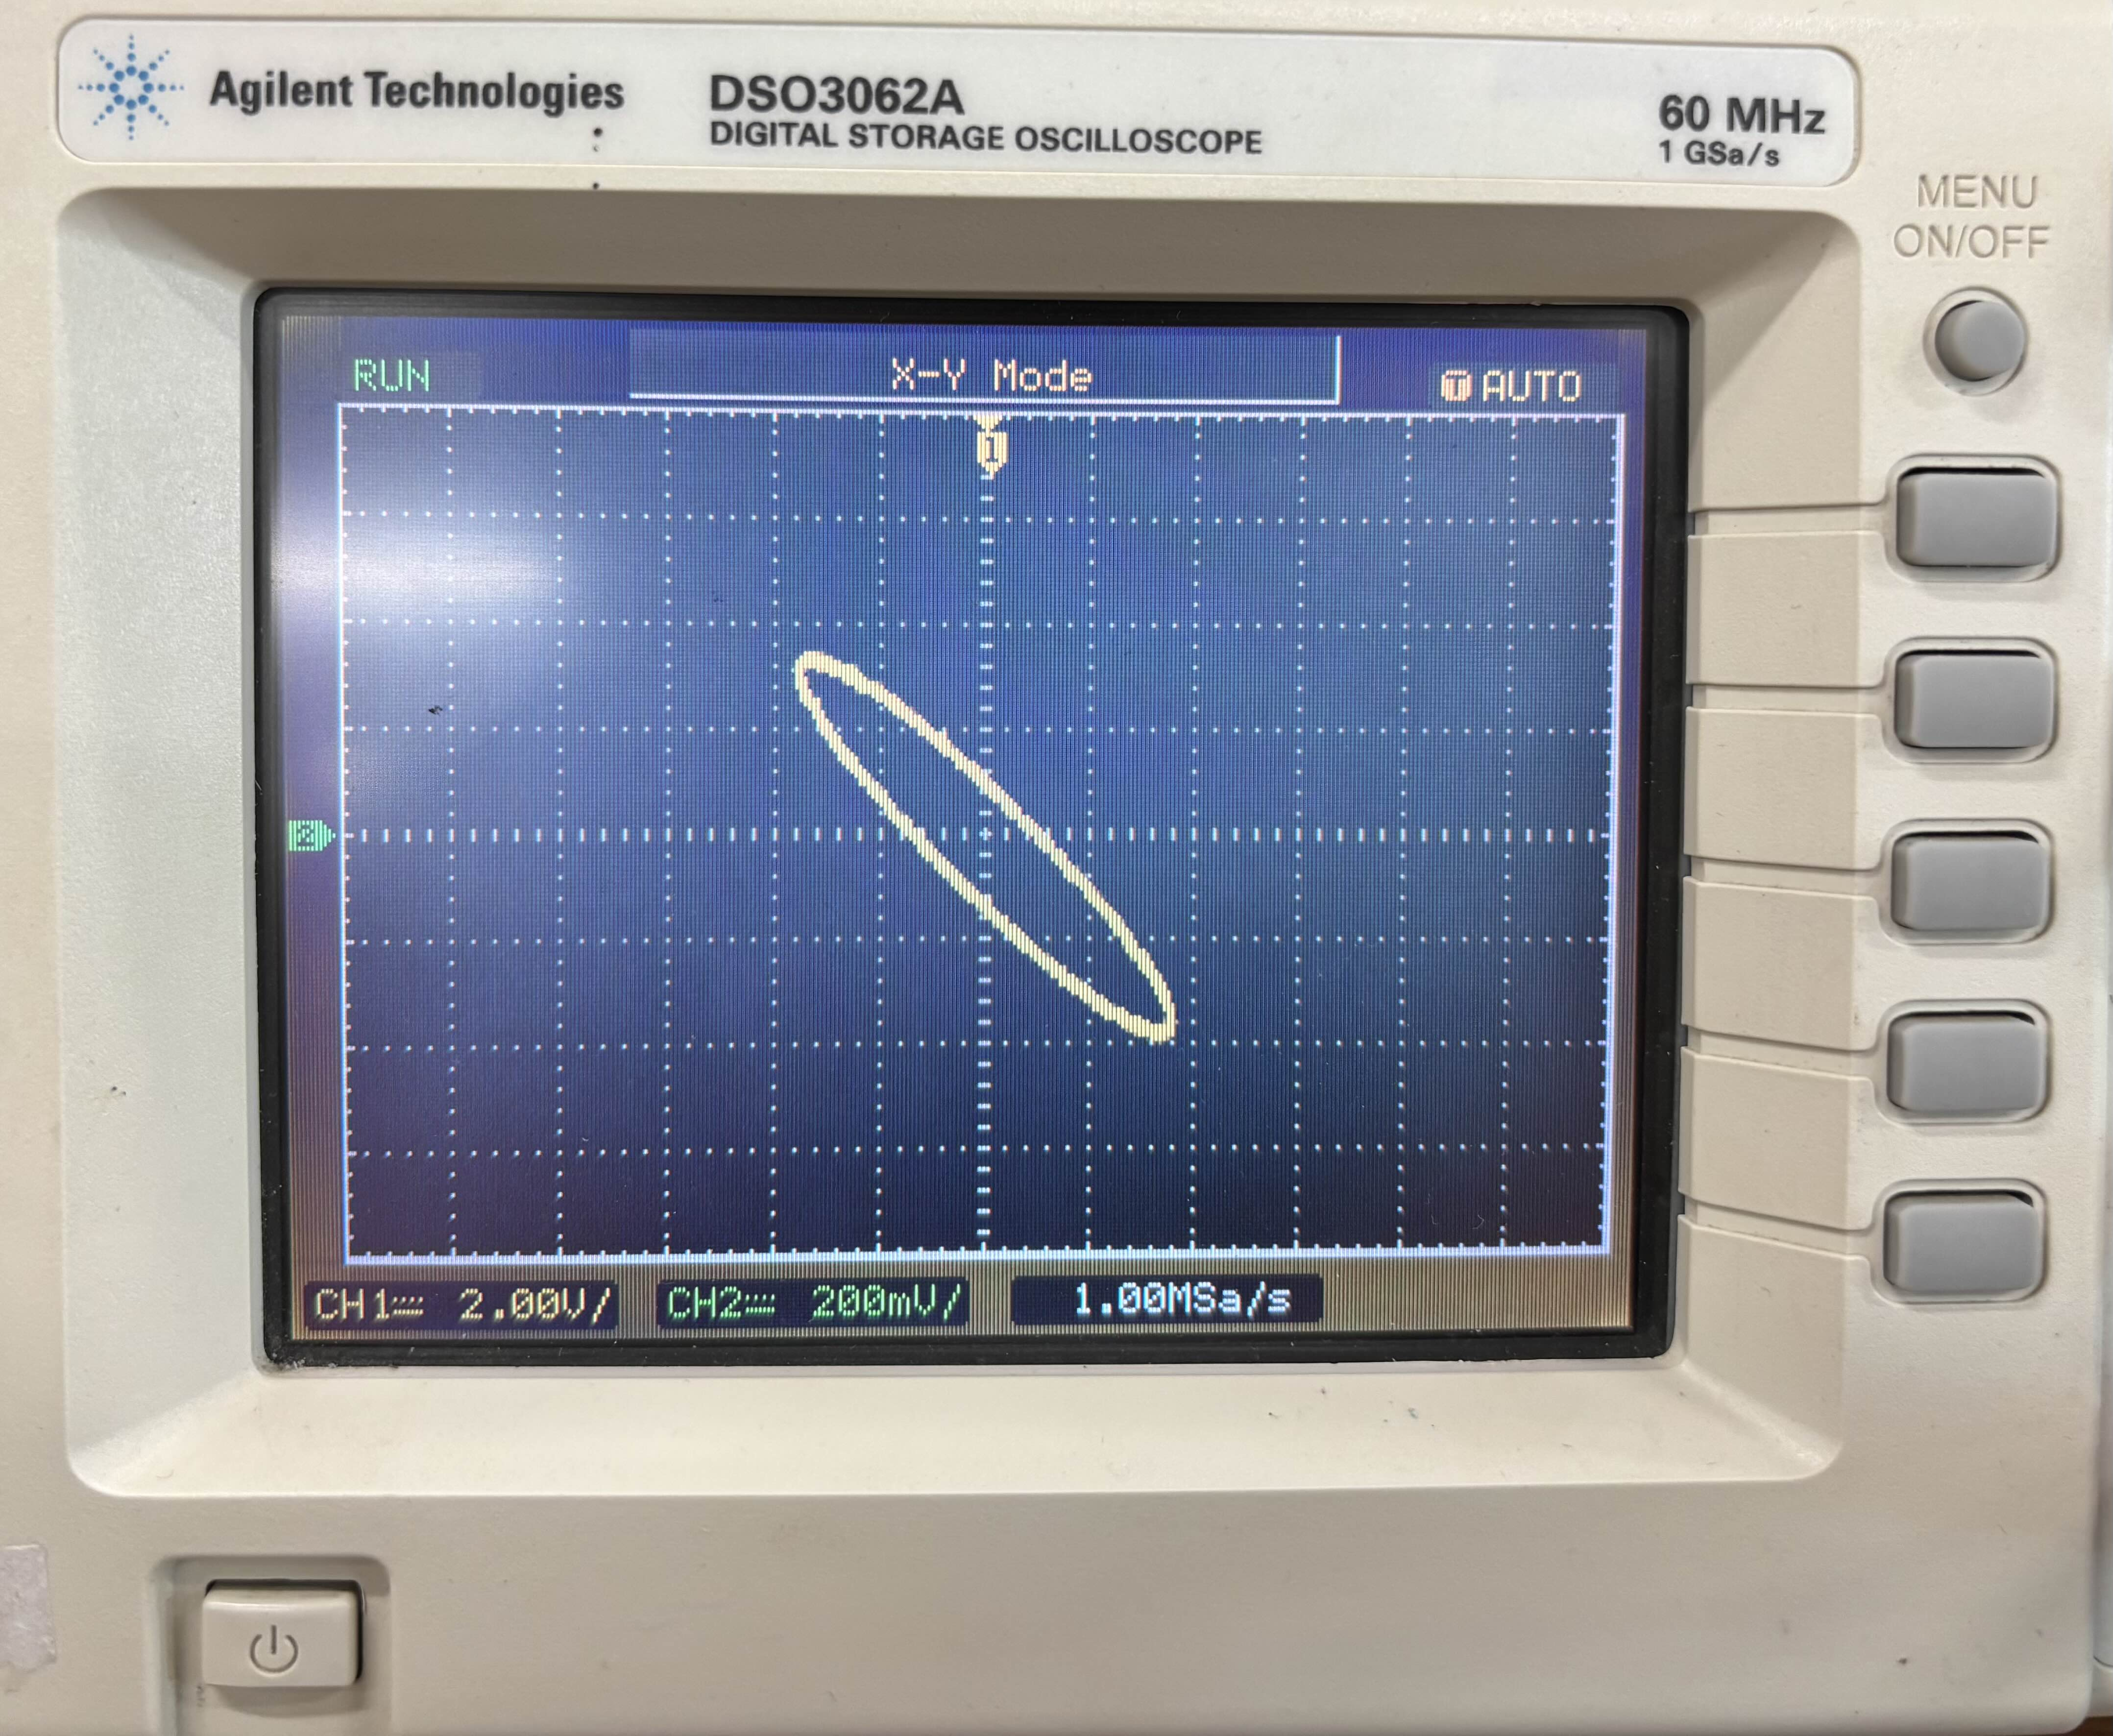
\includegraphics[width = 150pt]{figs/fig3_1.jpeg}
	\end{subfigure}
	\caption{Lissajous Figure 3}
\end{figure}
	\pagebreak
	\item $x(t) = 13\sin(6000\pi\omega t + \frac{\pi}{2})$, $y(t) = 5\sin(32000\pi\omega t + \frac{31\pi}{36})$\\
\begin{figure}[h!]
	\begin{subfigure}[b]{10pt}
		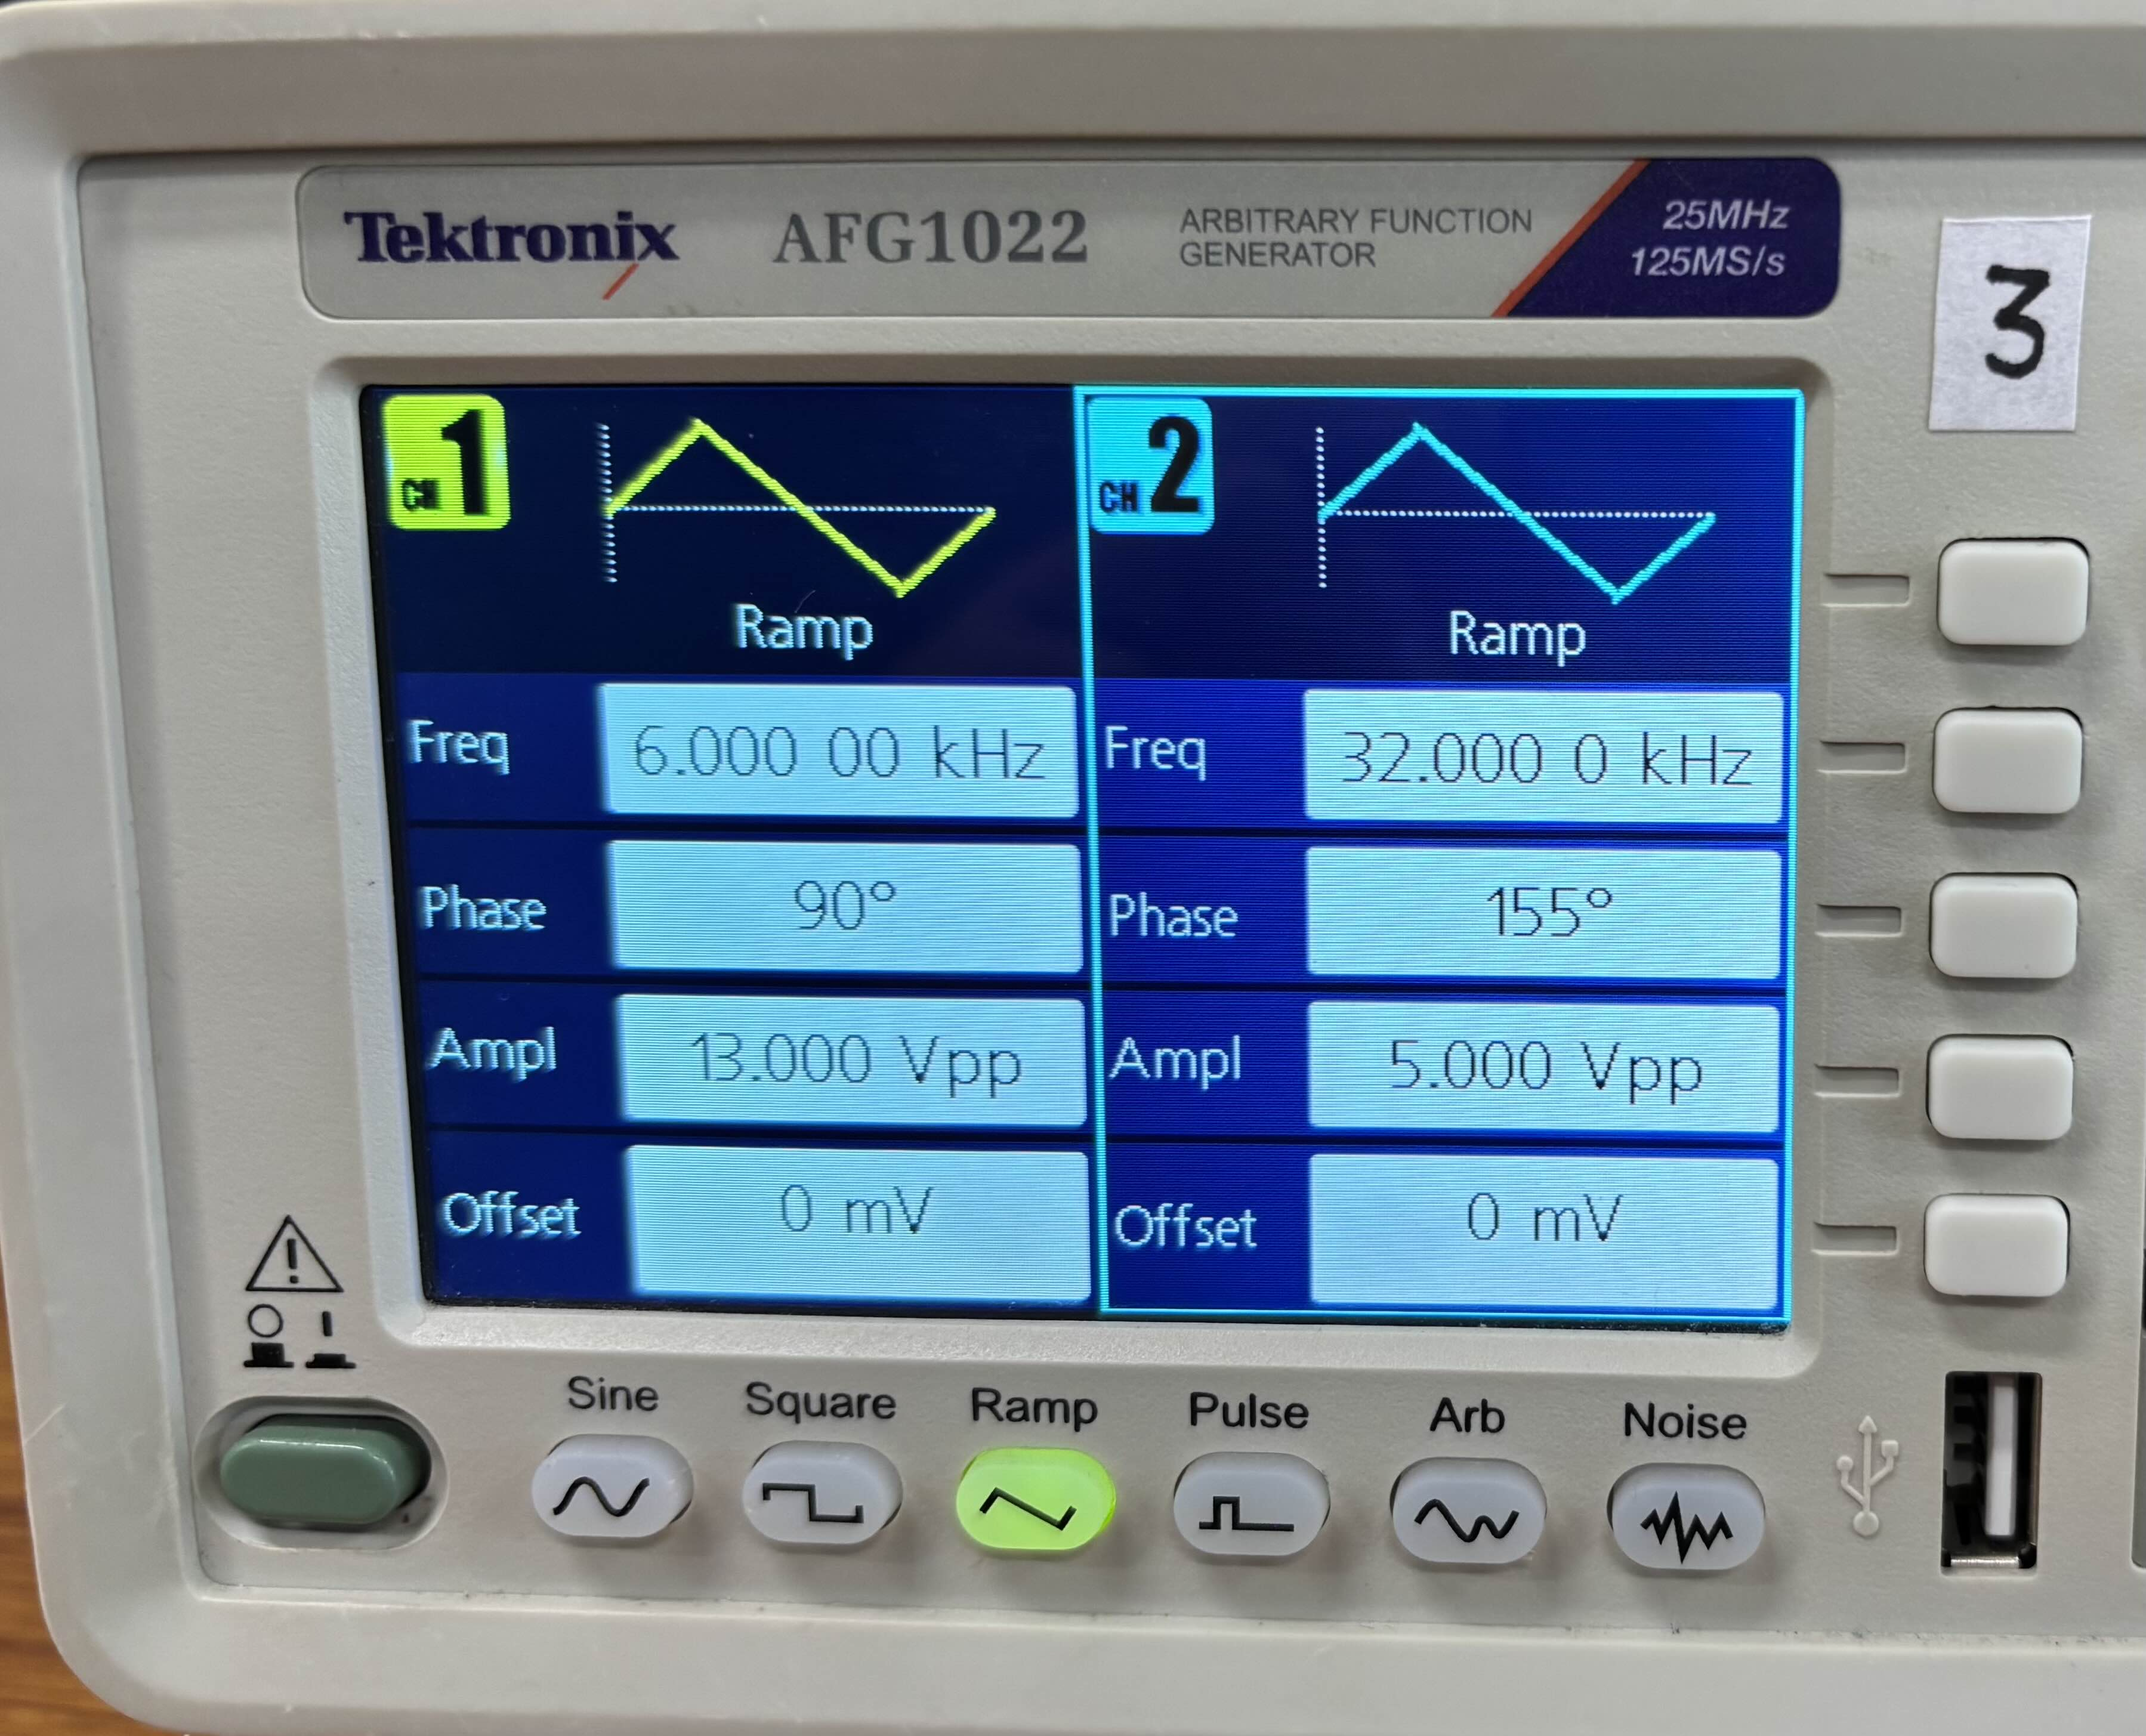
\includegraphics[width = 150pt]{figs/fig4.jpeg}
	\end{subfigure}
	\hspace{135pt}
	\begin{subfigure}[b]{10pt}
		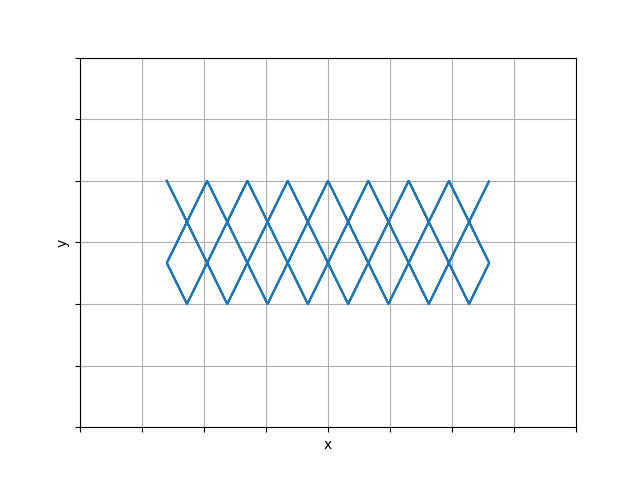
\includegraphics[width = 150pt]{figs/fig4.png}
	\end{subfigure}
	\hspace{135pt}
	\begin{subfigure}[b]{10pt}
		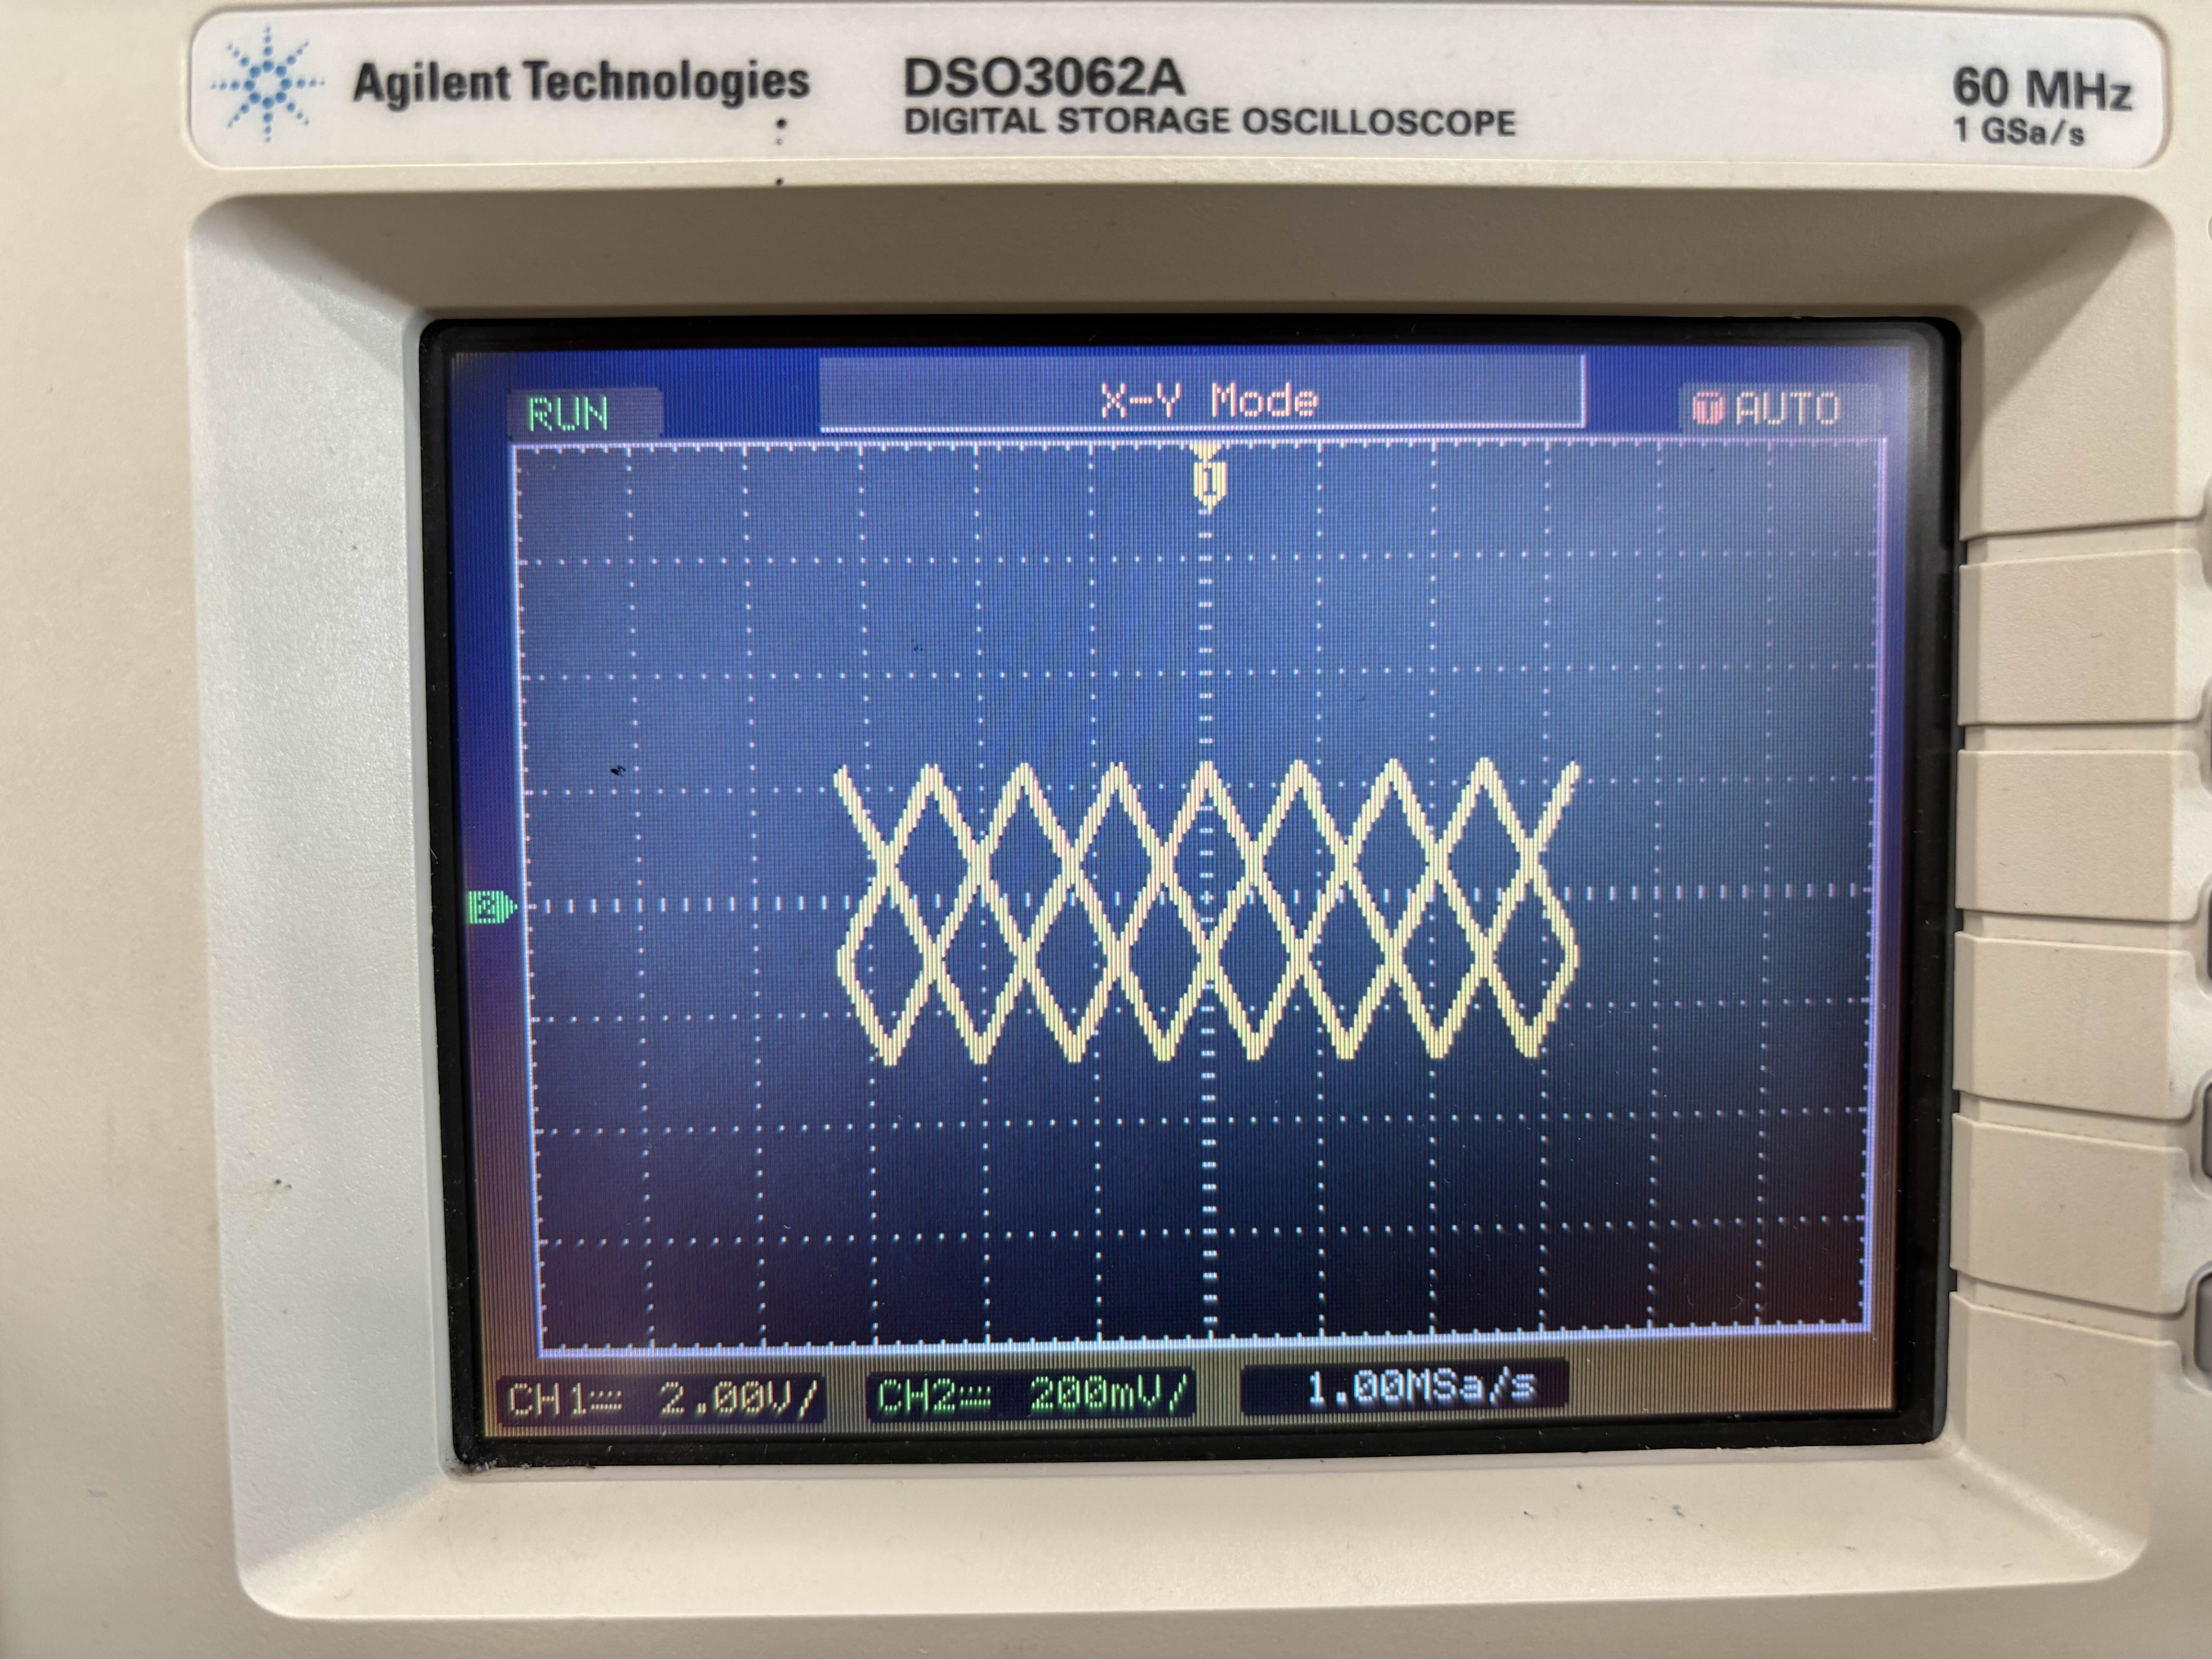
\includegraphics[width = 150pt]{figs/fig4_1.jpeg}
	\end{subfigure}
	\caption{Lissajous Figure 4}
\end{figure}
	\item $x(t) = 13\sin(6000\pi\omega t + \frac{\pi}{2})$, $y(t) = 5\sin(32000\pi\omega t + \frac{11\pi}{36})$\\
\begin{figure}[h!]
	\begin{subfigure}[b]{10pt}
		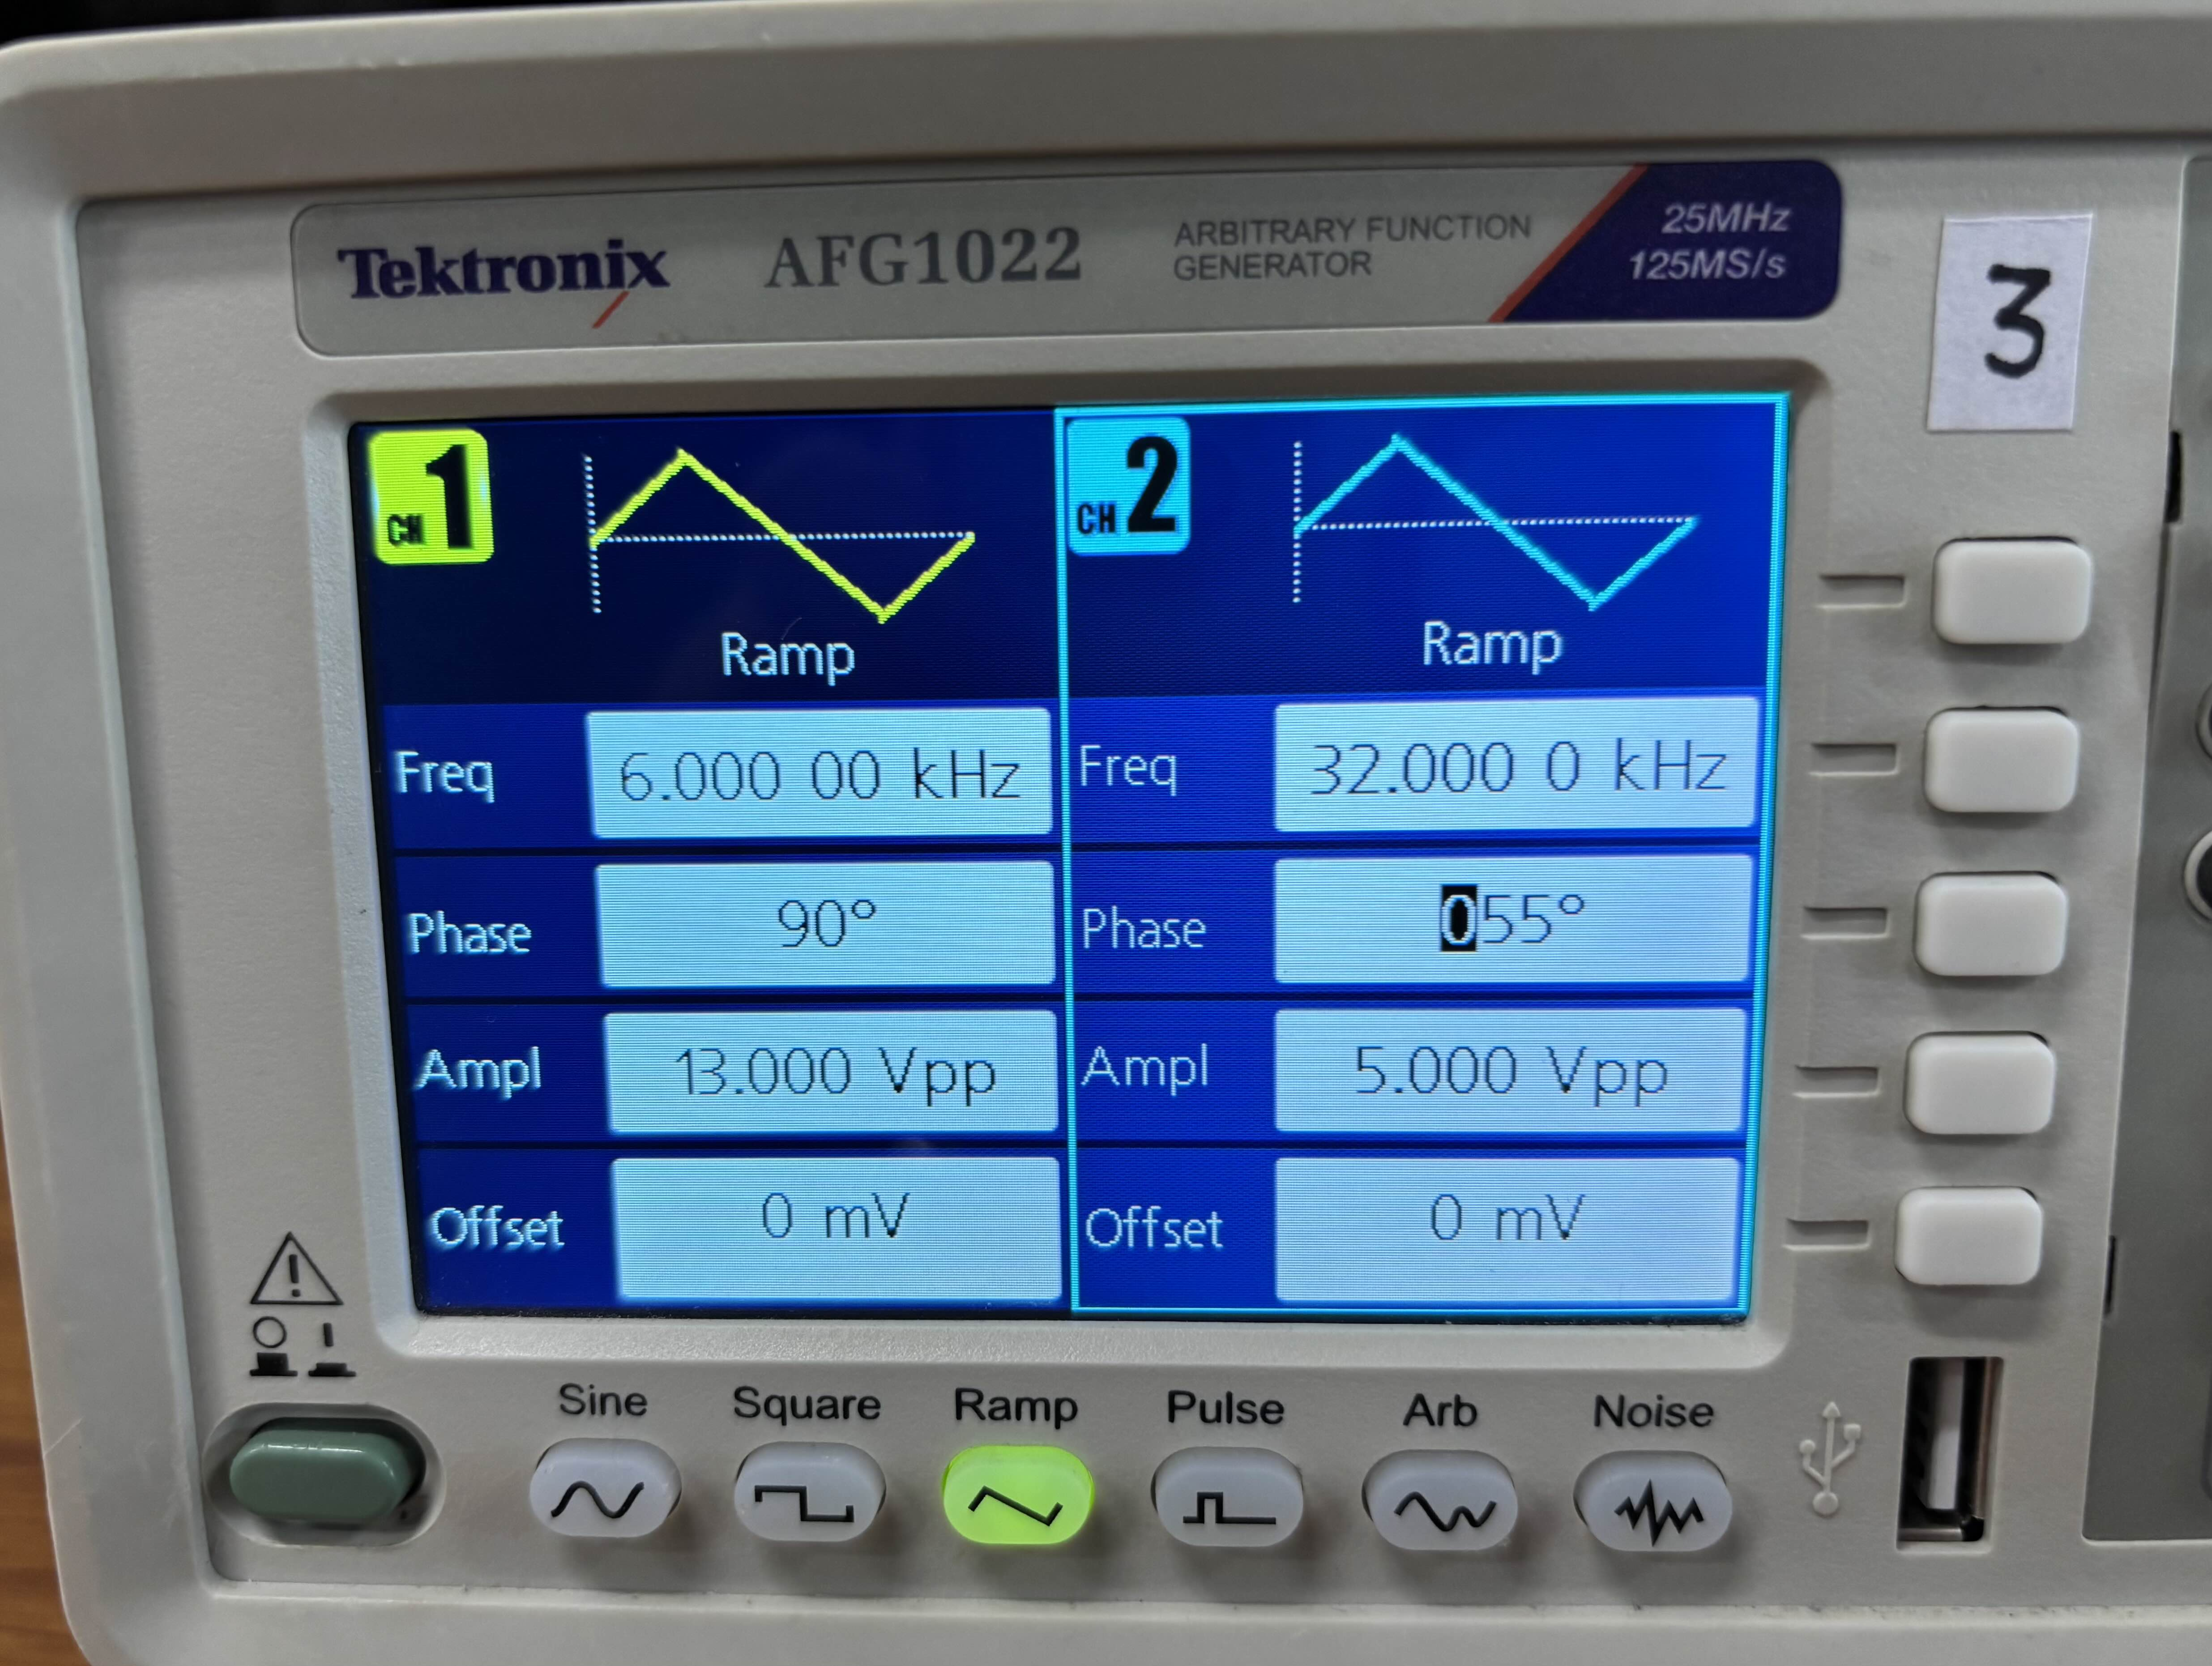
\includegraphics[width = 150pt]{figs/fig5.jpeg}
	\end{subfigure}
	\hspace{135pt}
	\begin{subfigure}[b]{10pt}
		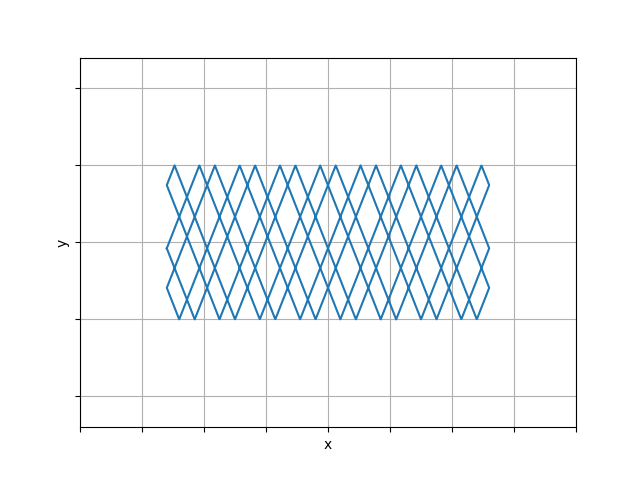
\includegraphics[width = 150pt]{figs/fig5.png}
	\end{subfigure}
	\hspace{135pt}
	\begin{subfigure}[b]{10pt}
		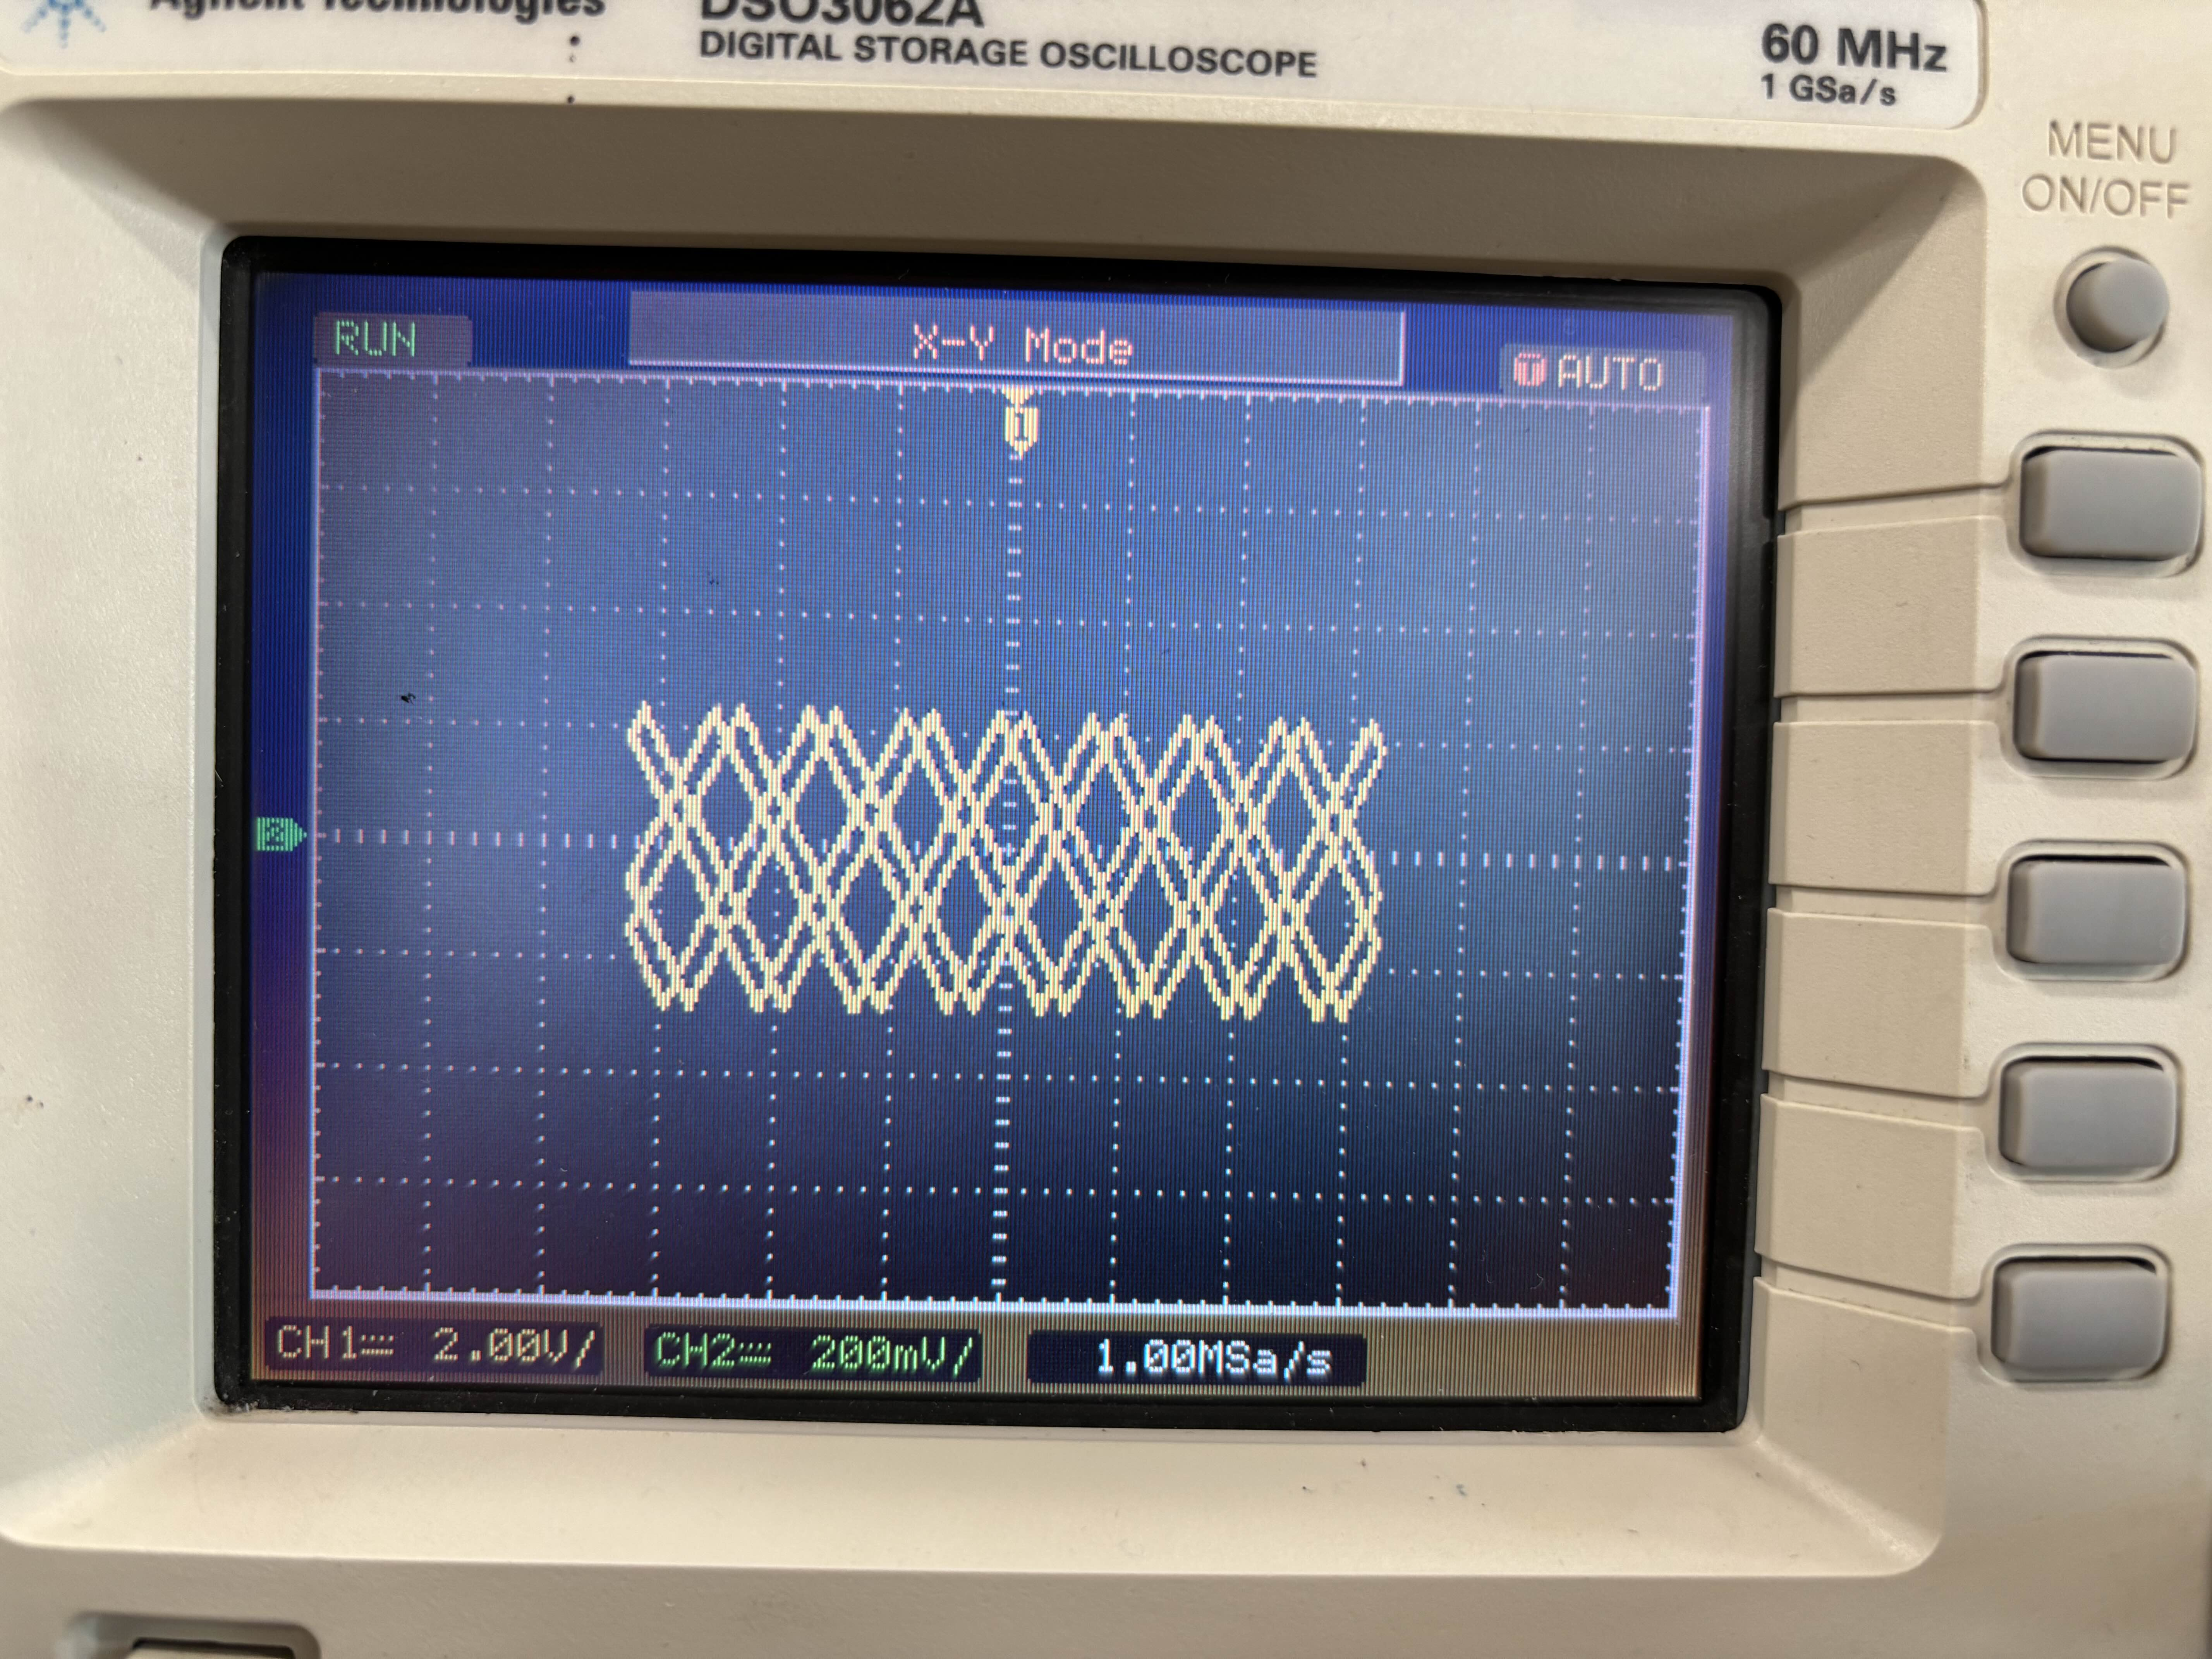
\includegraphics[width = 150pt]{figs/fig5_1.jpeg}
	\end{subfigure}
	\caption{Lissajous Figure 5}
\end{figure}
	\item $x(t) = 13\sin(1000\pi\omega t + \frac{\pi}{3})$, $y(t) = 4\sin(2000\pi\omega t + \frac{\pi}{12})$\\
\begin{figure}[h!]
	\begin{subfigure}[b]{10pt}
		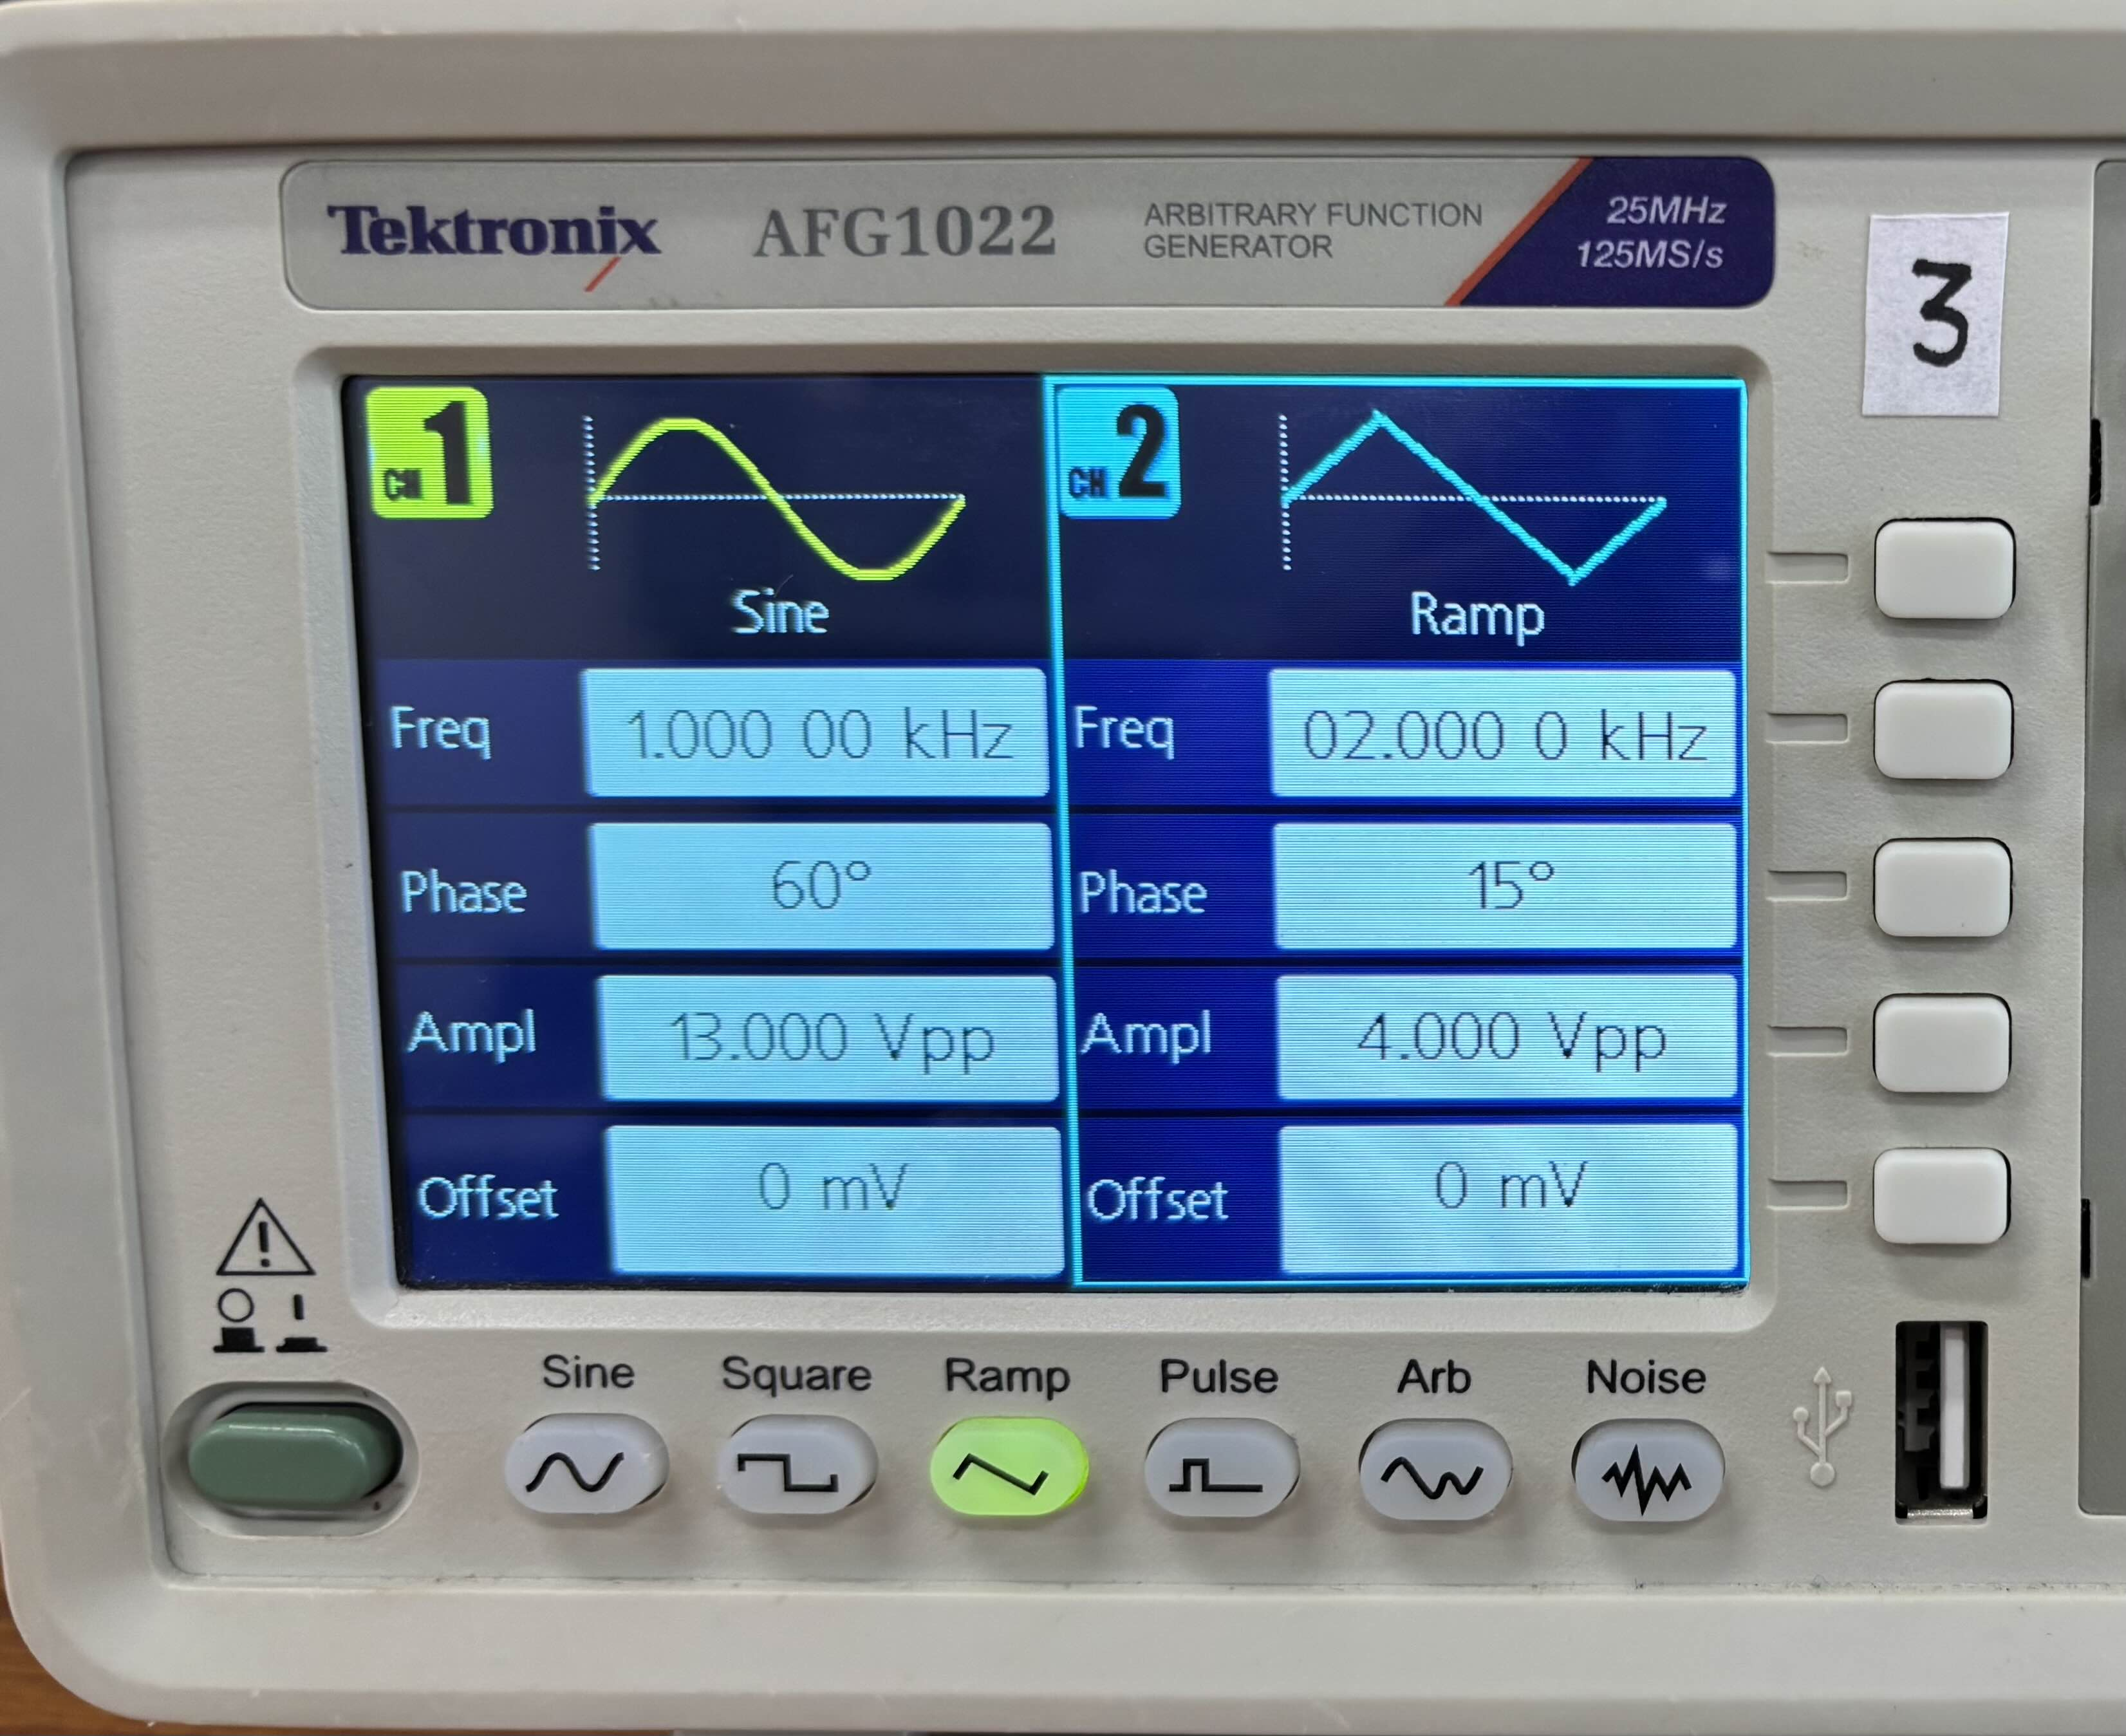
\includegraphics[width = 150pt]{figs/fig6.jpeg}
	\end{subfigure}
	\hspace{135pt}
	\begin{subfigure}[b]{10pt}
		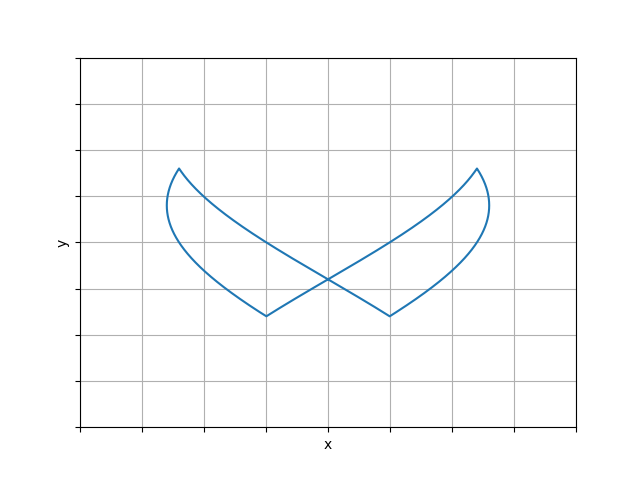
\includegraphics[width = 150pt]{figs/fig6.png}
	\end{subfigure}
	\hspace{135pt}
	\begin{subfigure}[b]{10pt}
		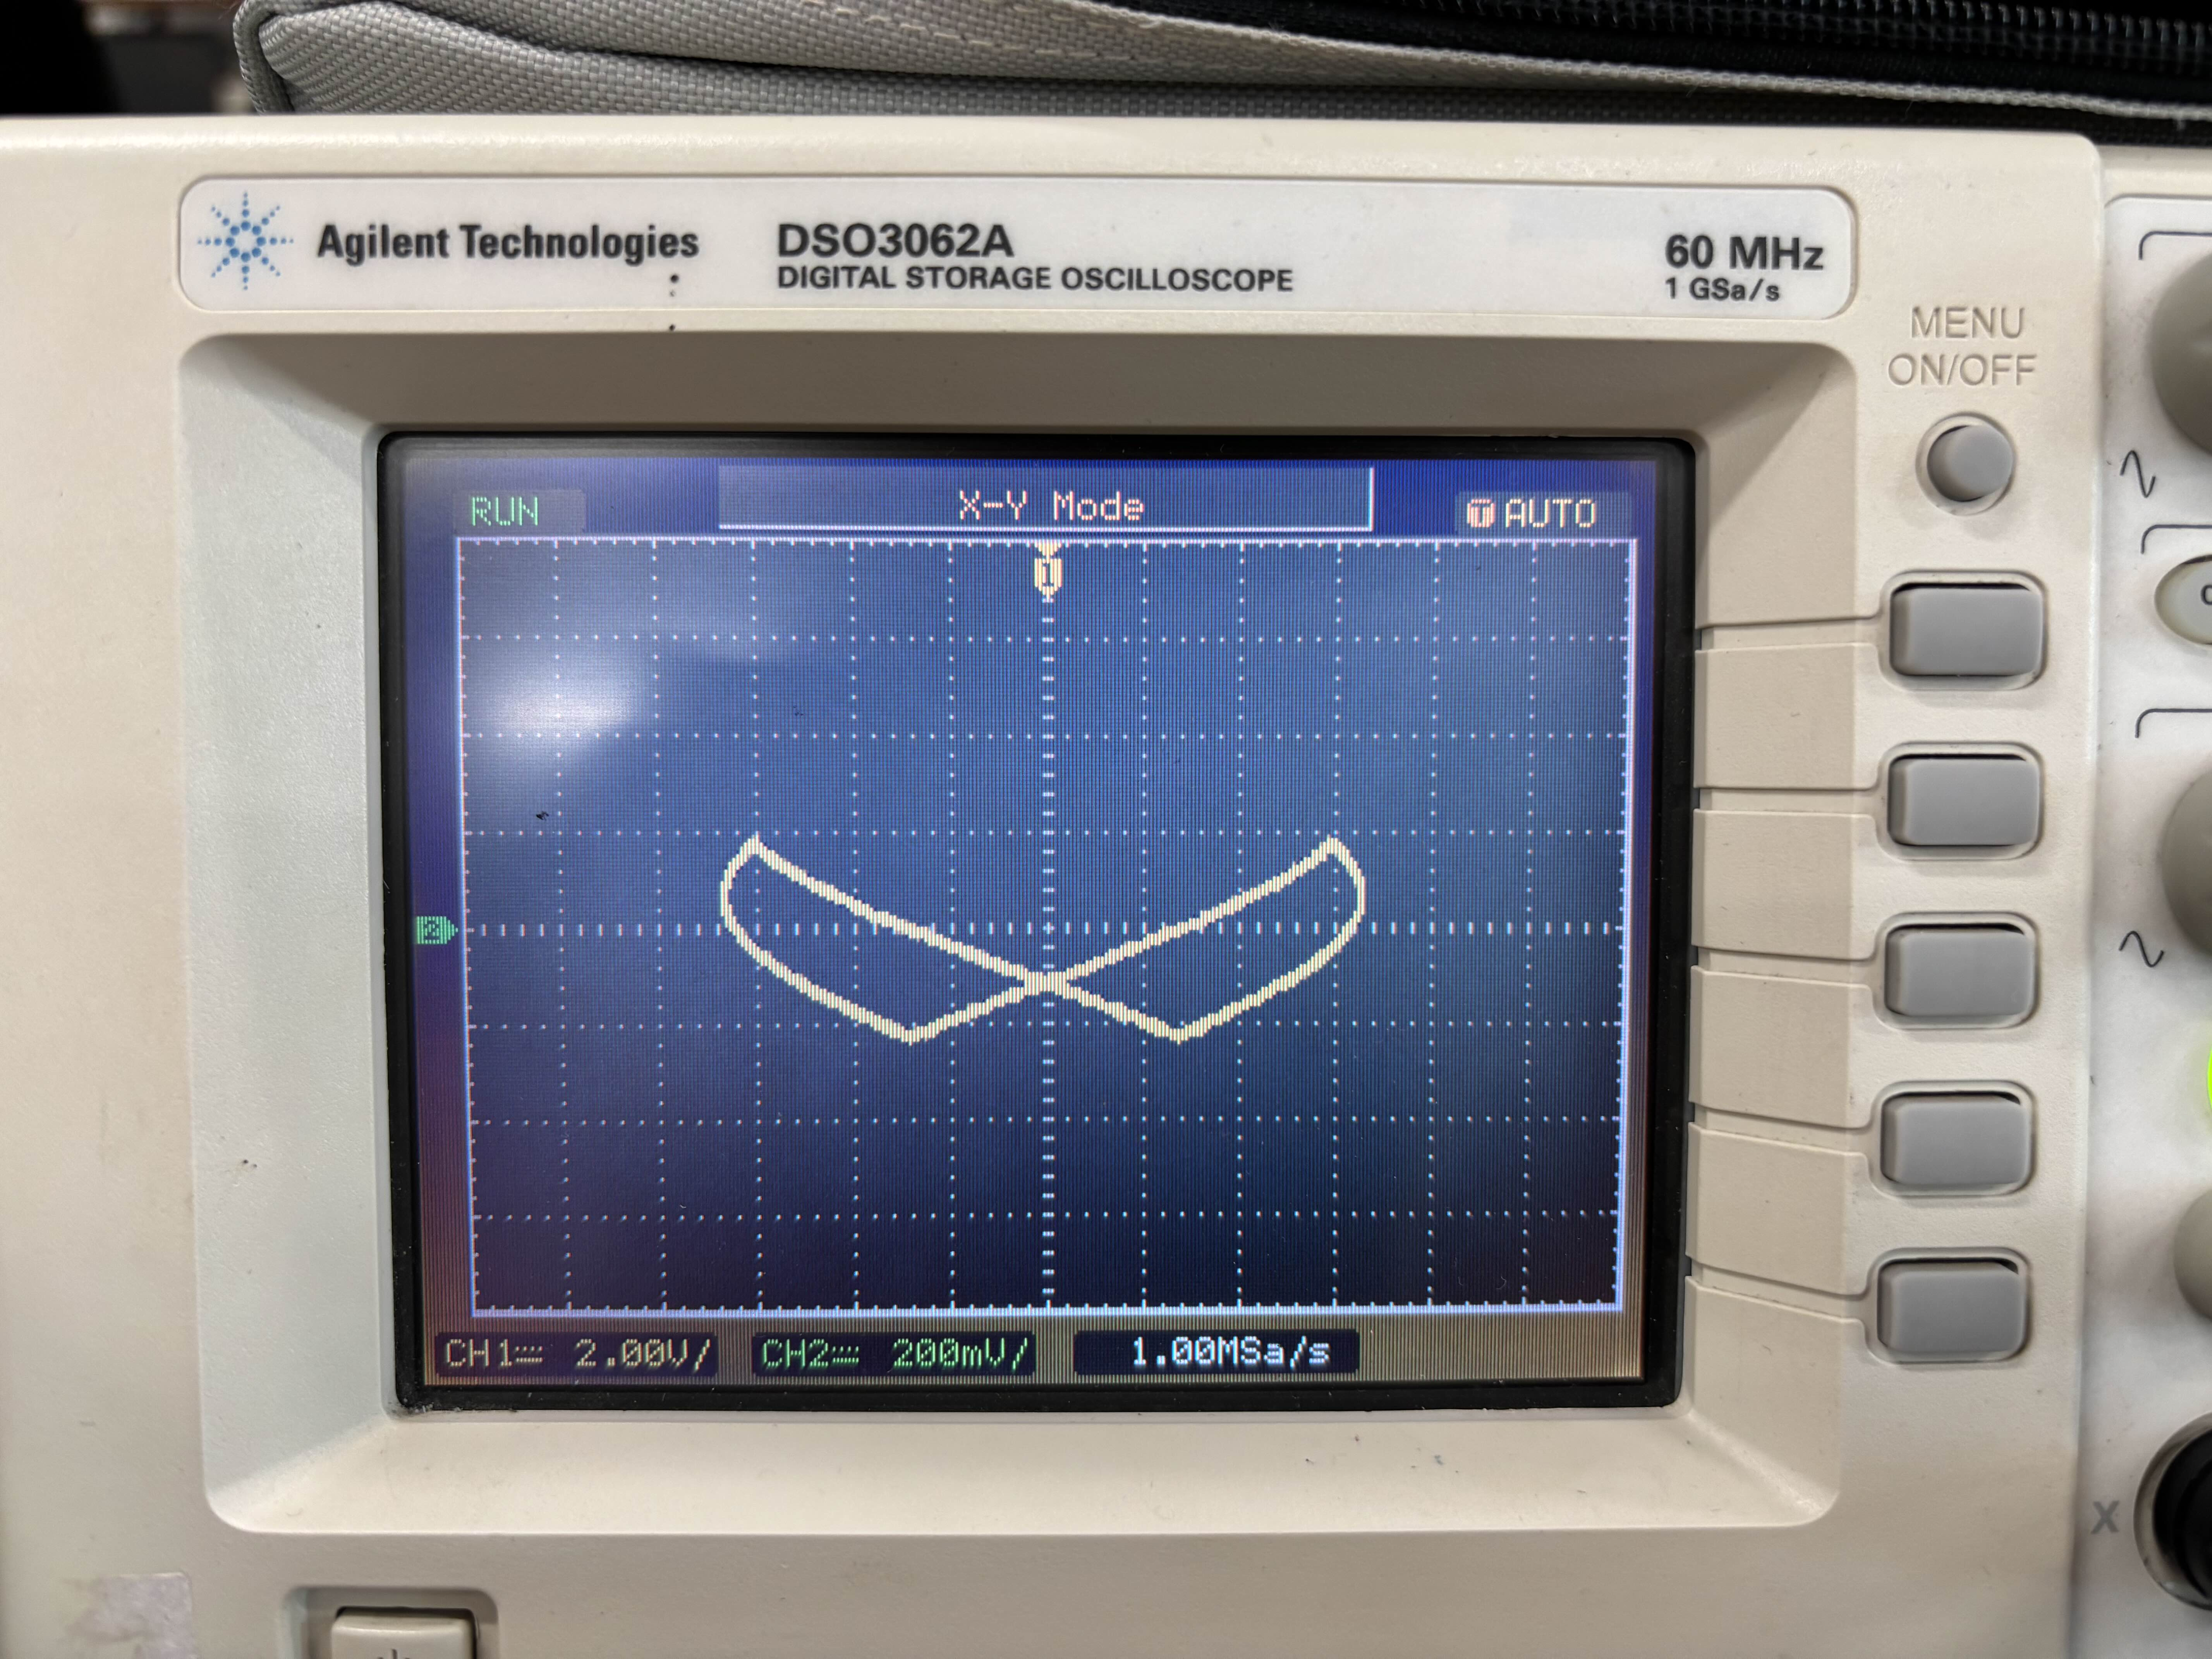
\includegraphics[width = 150pt]{figs/fig6_1.jpeg}
	\end{subfigure}
	\caption{Lissajous Figure 6}
\end{figure}
	\pagebreak
	\item $x(t) = 13\sin(2000\pi\omega t + \frac{\pi}{3})$, $y(t) = 4\sin(12000\pi\omega t + \frac{\pi}{12})$\\
\begin{figure}[h!]
	\begin{subfigure}[b]{10pt}
		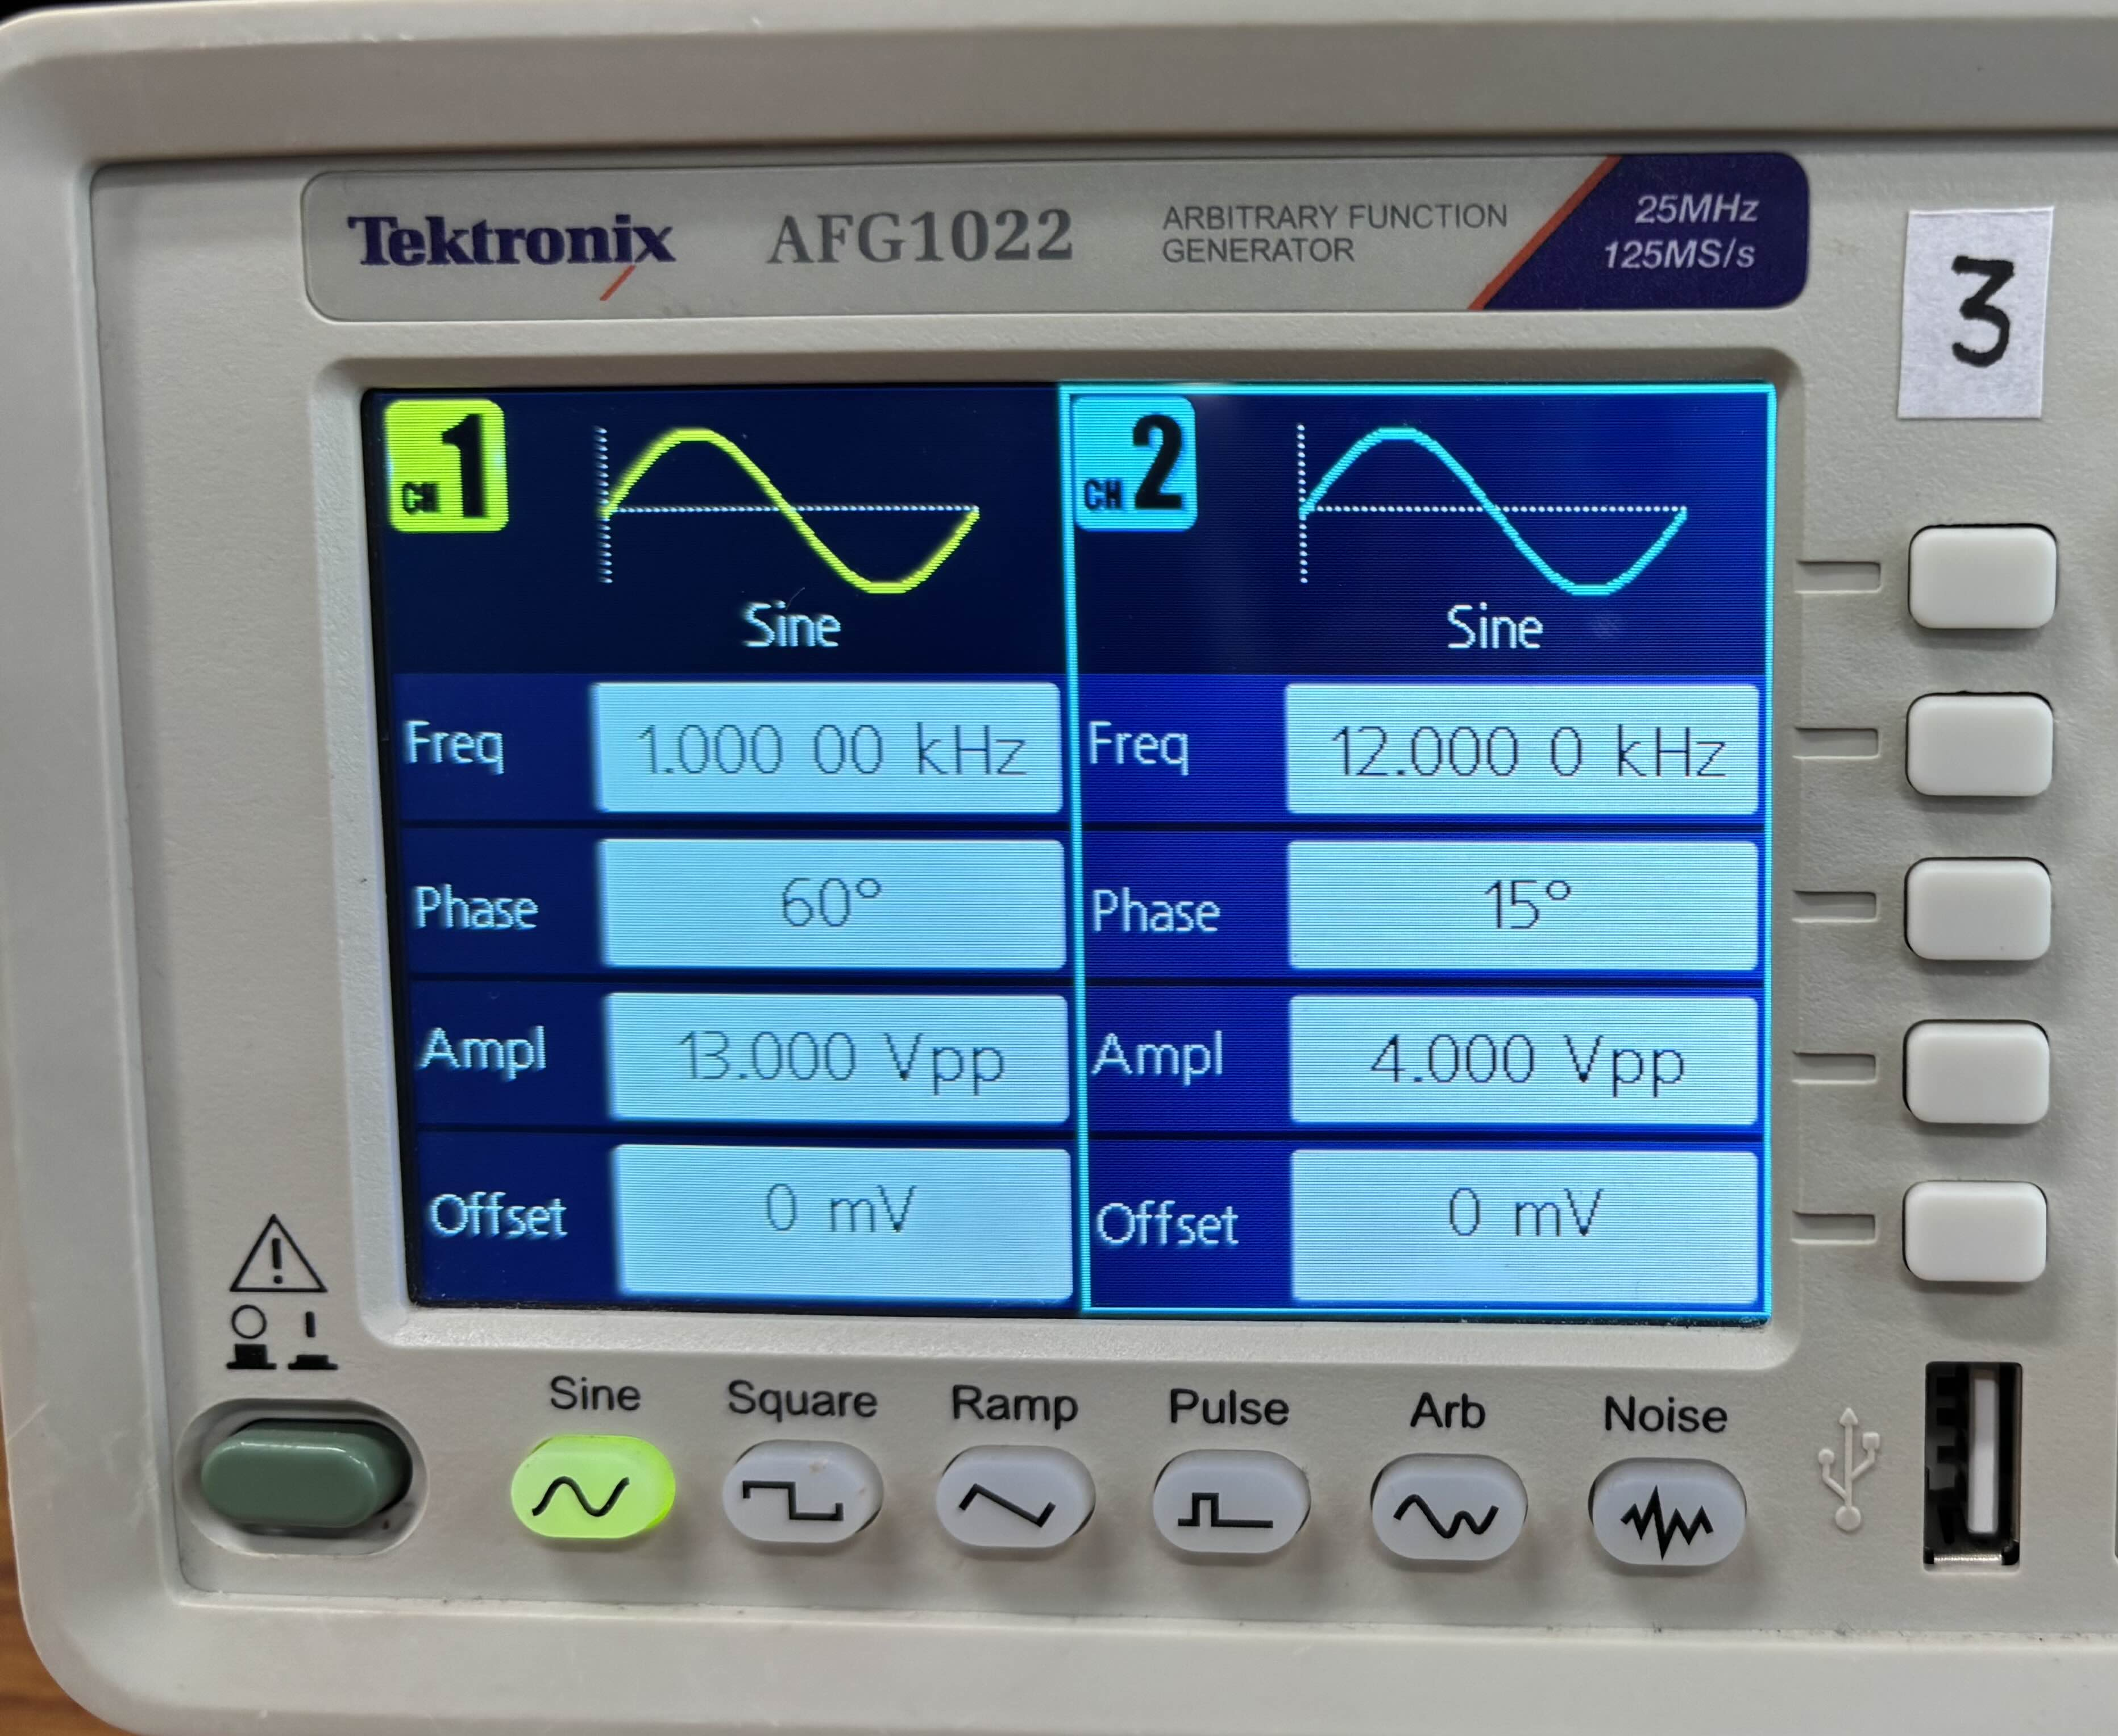
\includegraphics[width = 150pt]{figs/fig7.jpeg}
	\end{subfigure}
	\hspace{135pt}
	\begin{subfigure}[b]{10pt}
		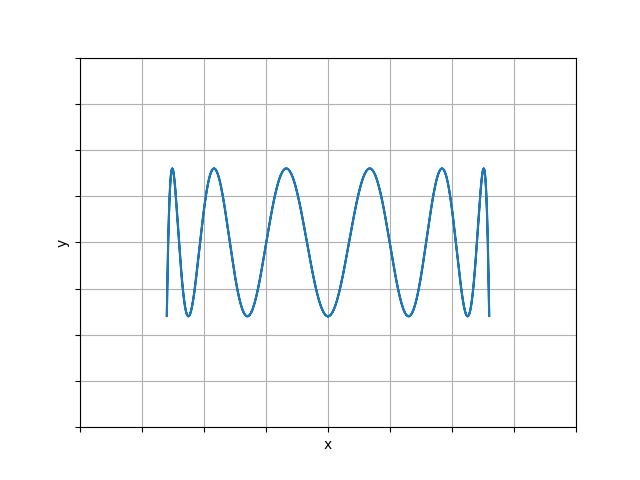
\includegraphics[width = 150pt]{figs/fig7.png}
	\end{subfigure}
	\hspace{135pt}
	\begin{subfigure}[b]{10pt}
		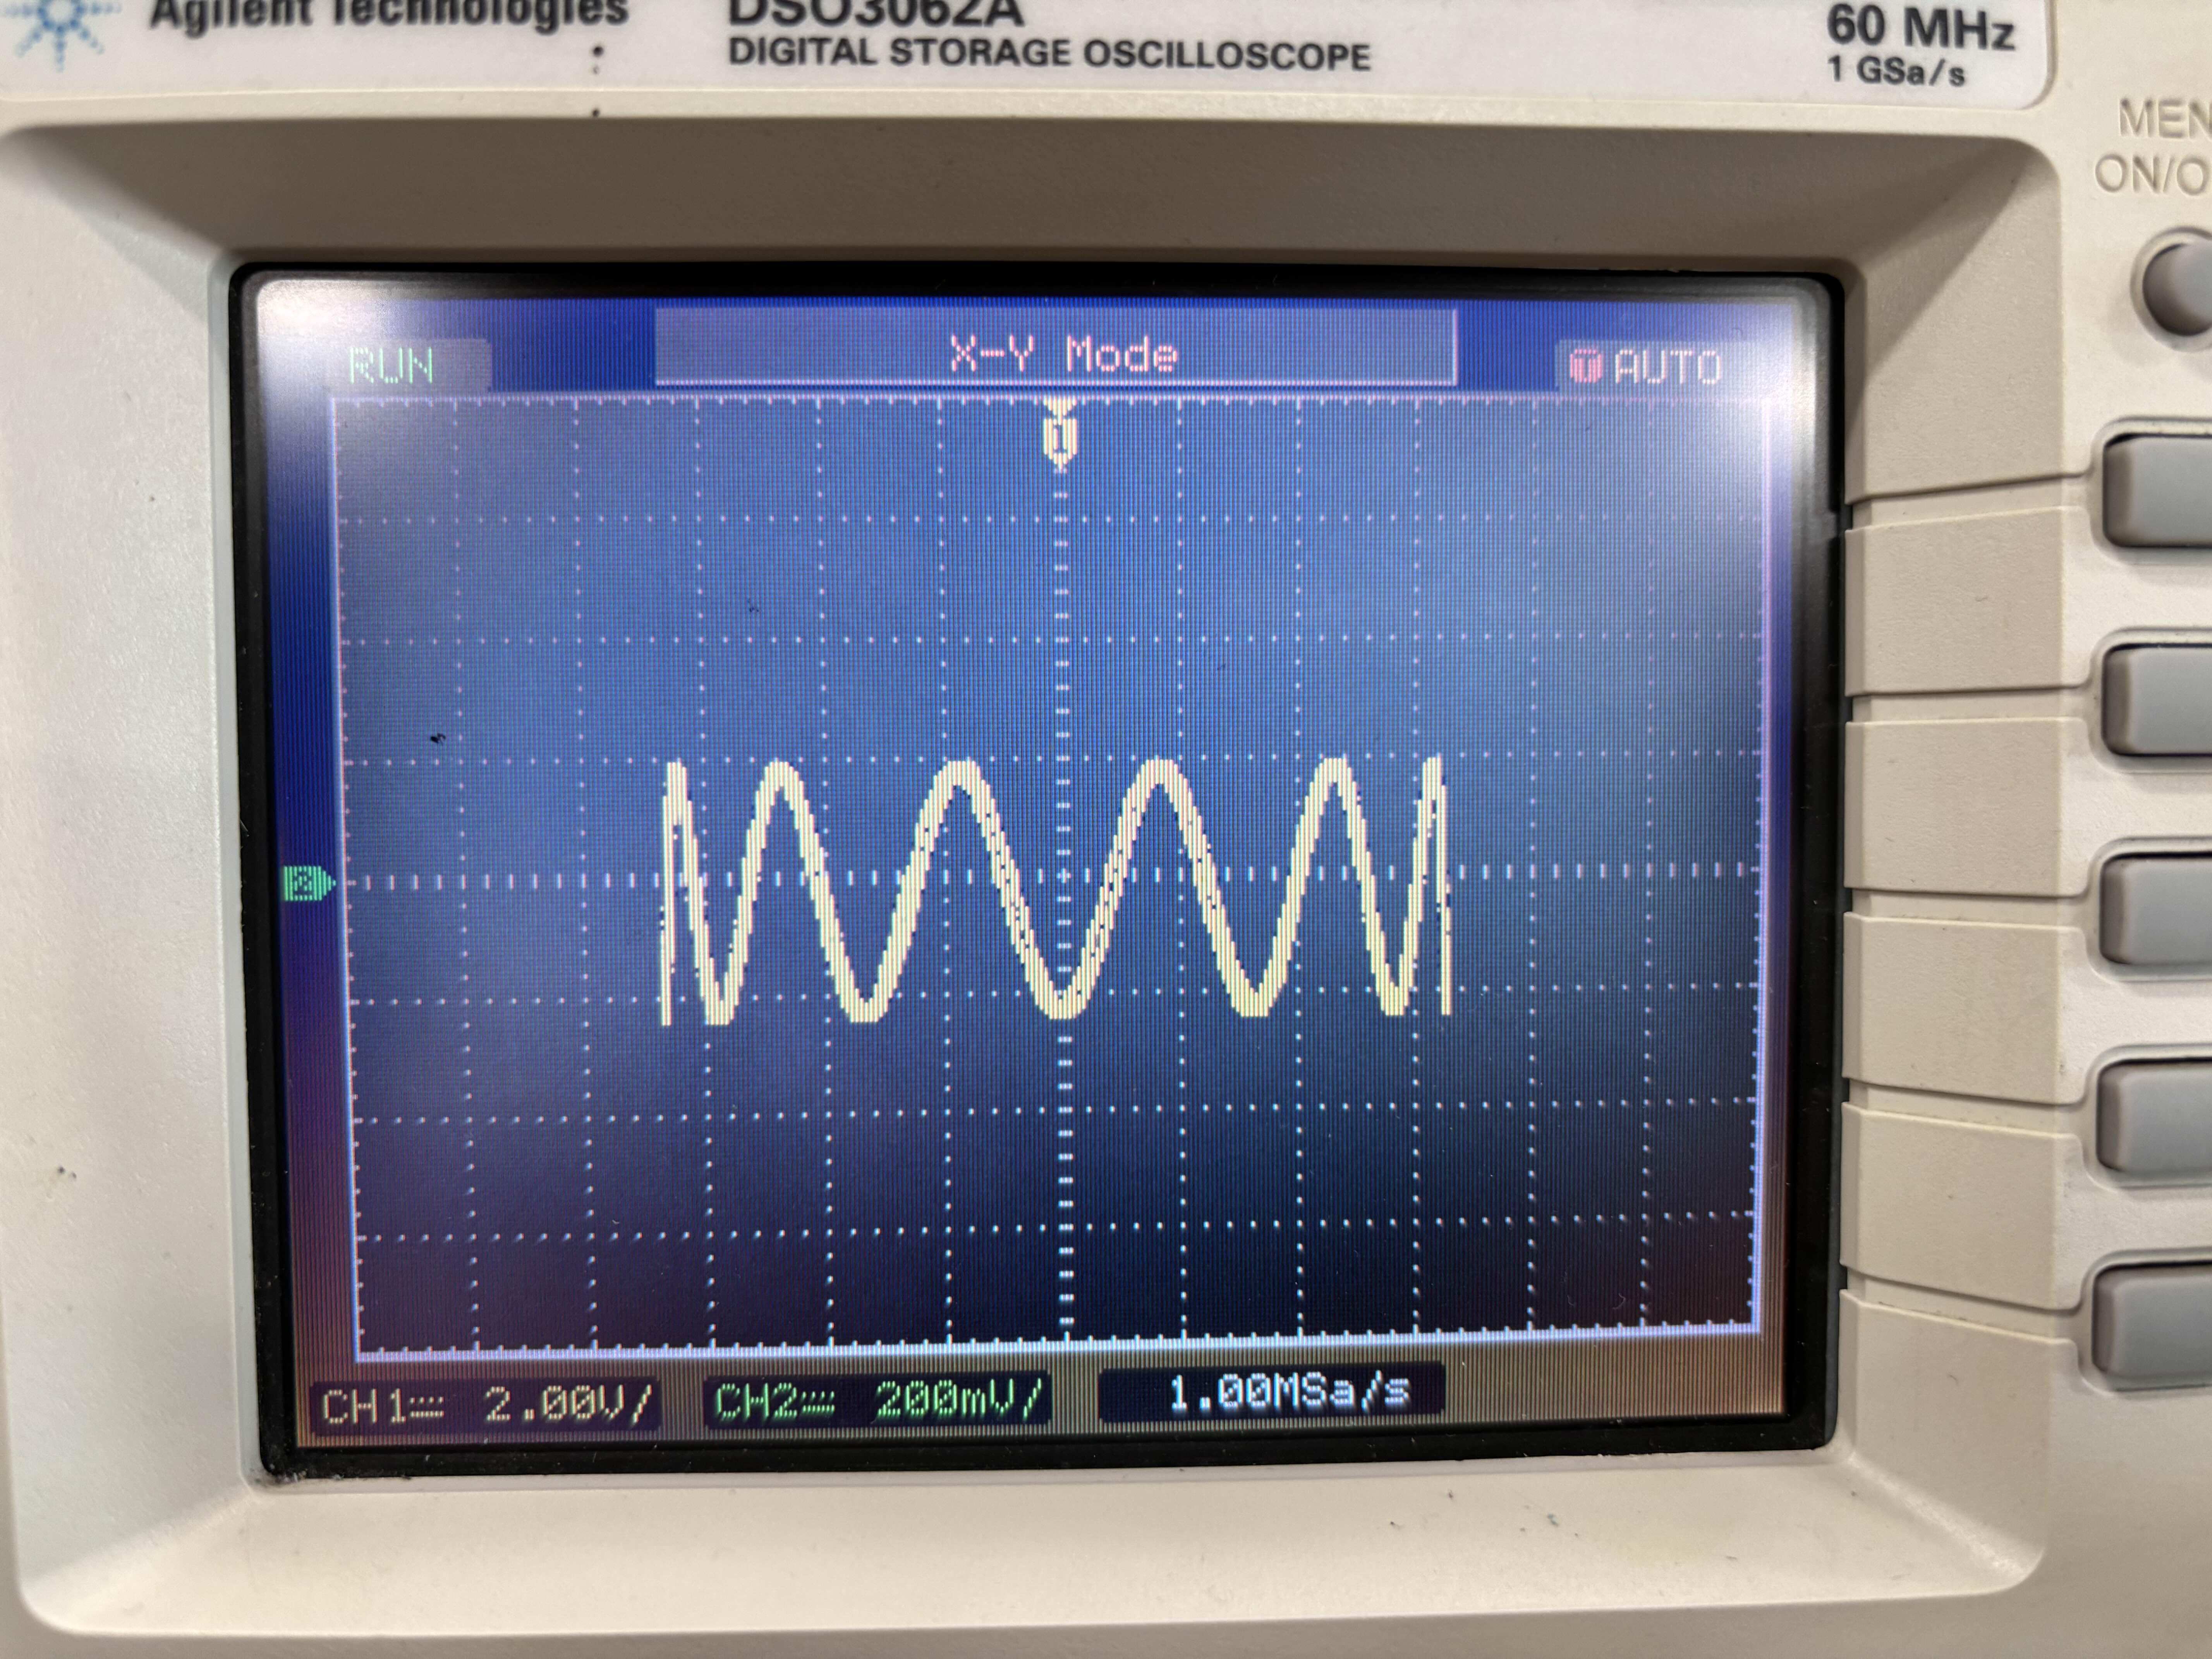
\includegraphics[width = 150pt]{figs/fig7_1.jpeg}
	\end{subfigure}
	\caption{Lissajous Figure 7}
\end{figure}
\end{enumerate}
We see that all the python and oscilloscope plots match. Hence, the plots are accurate\\
Python code verification of Lissajous figures:\\
\fbox{\url{https://github.com/ArjunPavanje/EE1200/tree/main/Experiment_1/codes}}

\subsection*{One-Time Event Capture}
The \texttt{Single} mode on the \text{oscilloscope} ensures that the display is frozen after capturing the first trigger event. This is useful for observing transient signals or rare events. By using \text{burst mode} on the \text{function generator}, a precise number of cycles or a single waveform is generated and can be accurately captured.\\
In this case, we have used a square wave input of amplitude $5$ Vpp and have set the number of cycles to $5$.\\
Below is the plot for the one time event which was captured\\
\begin{figure}[h!]
   \centering
   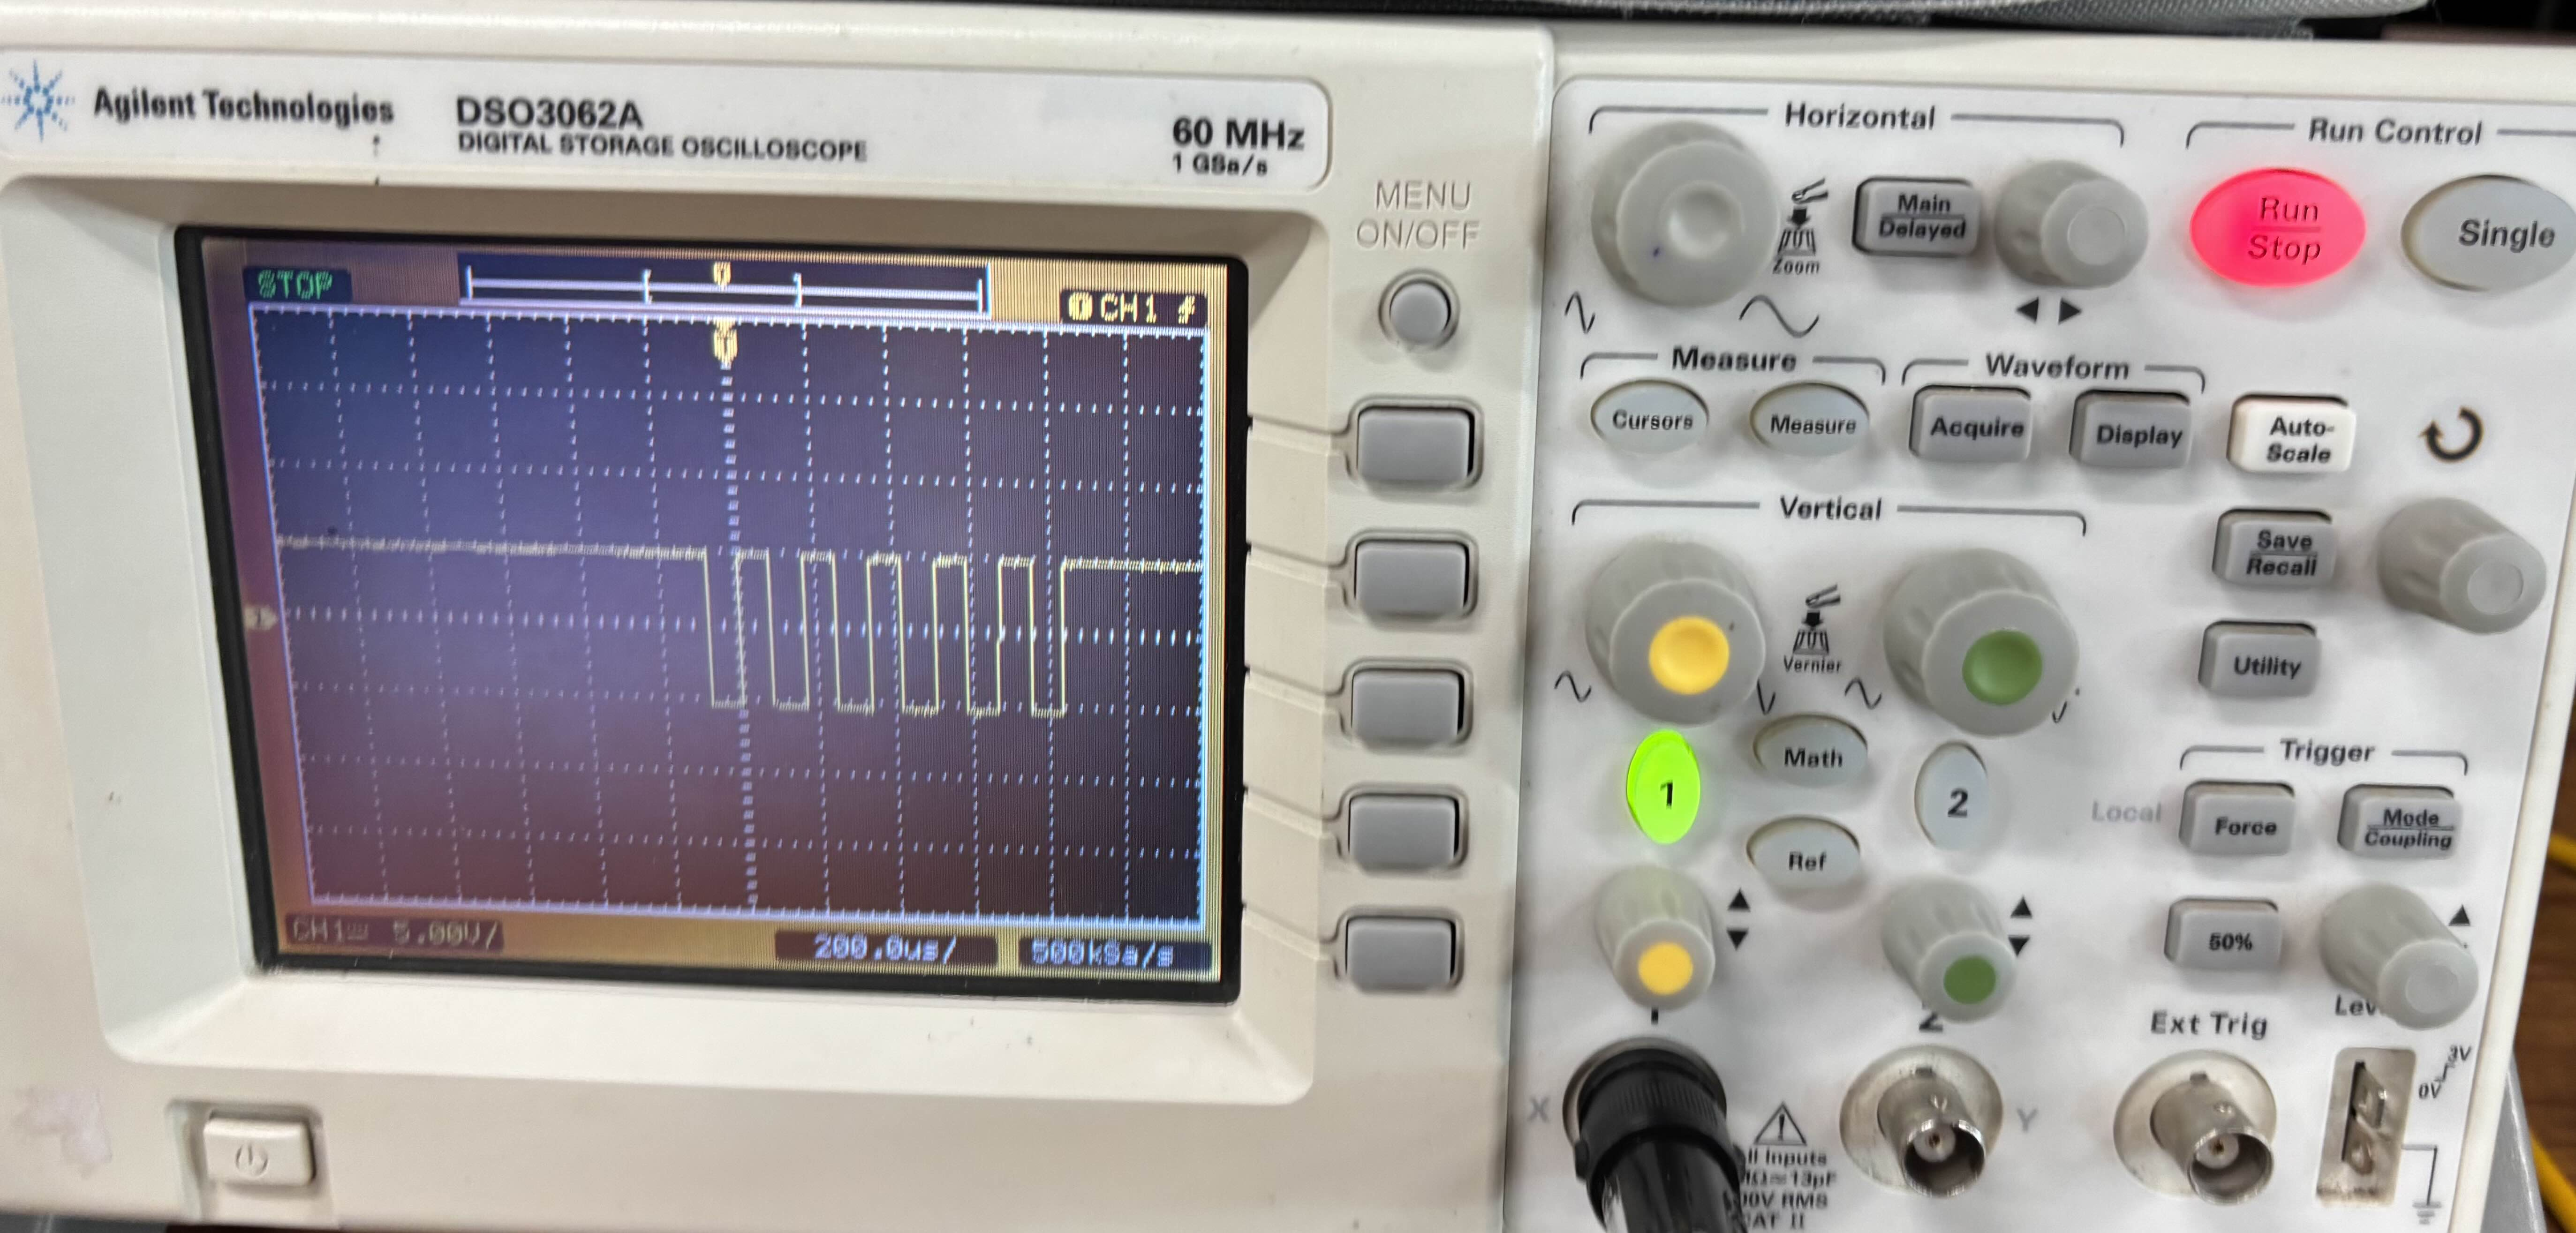
\includegraphics[width=300pt]{figs/one-time-event.jpeg}
   \caption{Capturing a one time event}
   \label{stemplot}
\end{figure}
\section*{Conclusion}
The experiment successfully demonstrated the generation and analysis of Lissajous figures, highlighting their dependence on frequency ratio and phase difference. The procedure to capture one-time events on a \text{oscilloscope} was also explored and verified using \text{burst mode} with manual triggering.

\end{document}
